\documentclass{article}
\usepackage{manualdoprofessor}
\usepackage{fichatecnica}
\usepackage{lipsum,media9,graficos}
\usepackage[justification=raggedright]{caption}
\usepackage{bncc}
\usepackage[lunna]{logoedlab}
\usepackage{marginnote}
 


\newcommand{\AutorLivro}{Lima Barreto}
\newcommand{\TituloLivro}{Crônicas e contos}
\newcommand{\Tema}{Ficção, mistério e fantasia}
\newcommand{\Genero}{Conto, crônica e novela}
% \newcommand{\imagemCapa}{PNLD0001-01.png}
\newcommand{\issnppub}{---}
\newcommand{\issnepub}{---}
% \newcommand{\fichacatalografica}{PNLD0001-00.png}
\newcommand{\colaborador}{\textit{Fulano de Tal} é uma pessoa incrível e vai fazer um bom serviço.}





\begin{document}



\title{\TituloLivro}
\author{\AutorLivro}
\def\authornotes{\colaborador}

\date{}
\maketitle
\tableofcontents


\pagebreak

\section{Carta aos professores}

Caro educador / Cara educadora,\\\bigskip

\reversemarginpar
\marginparwidth=5cm

\marginnote{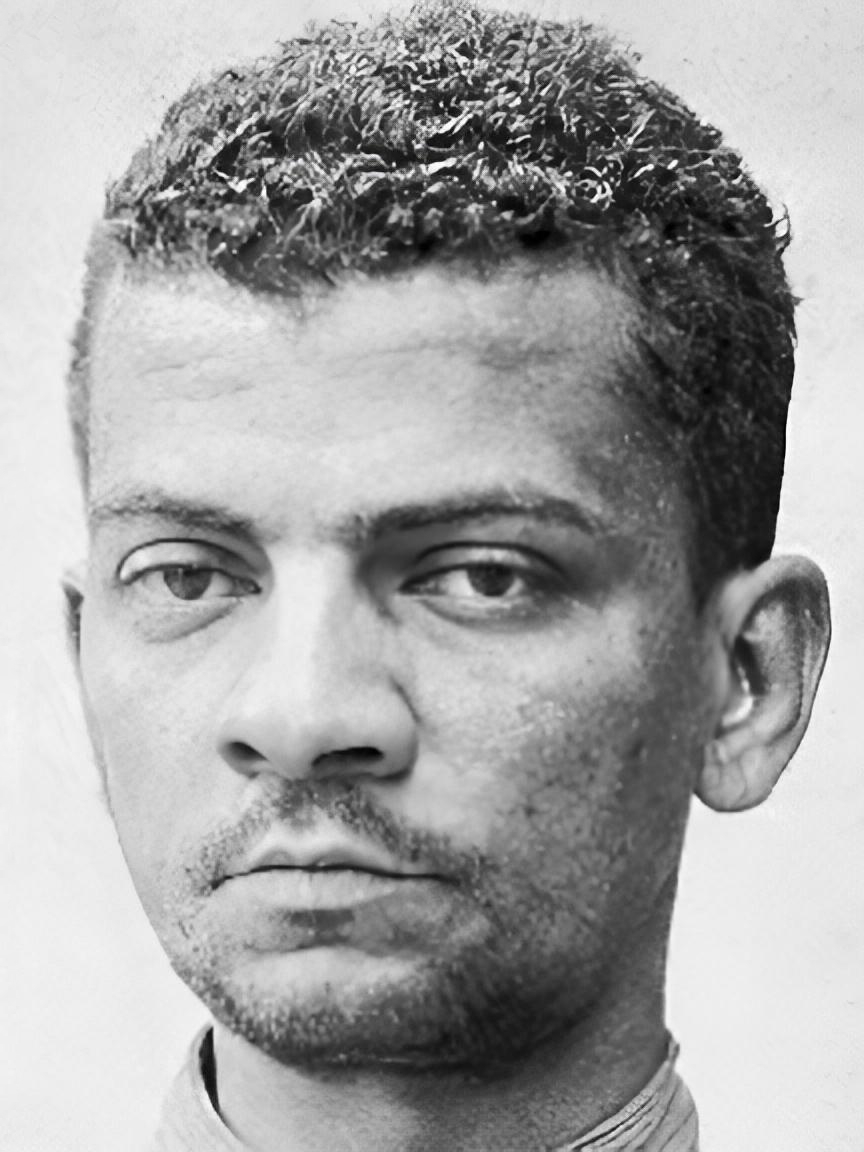
\includegraphics[width=5cm]{./images/PNLD0001-03.png}\\
\textit{Foto do autor}}


\publisheraddress

O presente manual tem por objetivo construir um apoio pedagógico entre a
\emph{Antologia de Crônicas e Contos de Lima Barreto} e aqueles e
aquelas para quem o livro foi pensado e preparado: alunas e alunos do
Ensino Médio. A pessoa fundamental para o sucesso desse encontro é
justamente você, educadora e educador, a quem convidamos a mergulhar na
fascinante e atual prosa curta de um de nossos maiores escritores.

O volume que organizamos consiste num pequeno recorte na grande produção
de crônicas e contos de Lima Barreto, publicados quase que totalmente na
imprensa da época --- jornais e revistas. Nosso intuito foi o de
aproximar o escritor brasileiro ao público jovem, buscando textos que
apresentem uma fácil compreensão, leitura fluida e que dialoguem com as
questões contemporâneas importantes para essa faixa etária.

A linguagem da crônica permitirá uma leitura mais agradável, menos
densa, embora necessitando de contextualização em muitos casos. Isso, no
entanto, pode ser um bom pretexto para a prática de atividades
incipientes de pesquisa textual e histórica. A organização das crônicas
em pequenos conjuntos temáticos teve como objetivo possibilitar a
realização de trabalhos e atividades continuadas, principalmente pelo
fato de apresentarem questões relevantes para os dias atuais.

A linguagem dos contos, além de suscitar questões importantes para a
formação cidadã das alunas e dos alunos, possibilita a fruição do texto
enquanto obra de arte, como ficção. Vocês perceberão que muitos contos
são desenvolvimentos mais ficcionais de assuntos que o autor já havia
trabalhado no nível da crônica, do jornalismo.

Esperamos poder contribuir para o encontro dos e das estudantes do
Ensino Médio com esse escritor tão fundamental para compreendermos as
contradições e os dilemas da sociedade brasileira.

\section{Propostas de atividades 1}
%\BNCC{EM13LGG703}
\BNCC{EM13LGG704}
\BNCC{EM13LP16}
\BNCC{EM13LP36}
\BNCC{EM13LP44}

\paragraph{Tema} Aprendendo um pouco sobre a Crônica como gênero
  literário.


\paragraph{Conteúdo} Apresentação, leitura e compreensão de algumas
crônicas da seção ``Cotidiano e Vida nos Subúrbios''. O educador ou a
educadora pode escolher outros textos que considerarem mais pertinentes
para a atividade.


\paragraph{Objetivos} Apreciar junto aos alunos e alunas o gênero
literário ``crônica'' a partir dos textos {\textit{A carroça dos
cachorros}} e {\textit{As enchentes}.}


\reversemarginpar
\marginparwidth=3cm

\marginnote{\footnotesize\textbf{EM13LGG704}\\
Apropriar-se criticamente de processos de pesquisa e busca de informação, por meio de ferramentas e dos novos formatos de produção e distribuição do conhecimento na cultura de rede.}


\paragraph{Justificativa:} O gênero crônica se constitui como um dos mais
acessíveis para se iniciar os estudos literários. Questões como foco
narrativo, temática, personagens, desenvolvimento de argumentos,
dimensões de espaço/tempo, ficção/realidade, engajamento da escrita,
ponto de vista, entre outras, podem estar presentes nesse tipo de
composição. Muitos escritores e escritoras célebres na literatura
brasileira escreveram crônicas para os jornais e depois reuniram em
livros, como o próprio Lima Barreto, mas também Machado de Assis,
Graciliano Ramos, Clarice Lispector, Raquel de Queiroz. Além daqueles
escritores que foram ``cronistas profissionais'': Rubem Braga, Sérgio
Porto (Stanislaw Ponte Preta), Paulo Mendes Campos, entre outros.
Atualmente existem excelentes escritoras e escritores produzindo
crônicas de ótima qualidade: Luis Fernando Veríssimo, Antônio Prata,
Ferréz, Noemi Jaffe, Eliane Brum, Conceição Evaristo, entre muitas
outras e outros.


Com o desaparecimento do lugar que a literatura ocupava nos jornais e
revistas, a crônica ressurgiu, principalmente a partir dos anos 2000 em
diante, com o advento da internet e principalmente dos blogs, sites e
revistas eletrônicas. Neste sentido, torna"-se importante para os alunos
e alunas uma contextualização desse gênero literário, mas sobretudo
mostrar que ele ainda continua em sua forma plena, agora nas plataformas
digitais.


\paragraph{Metodologia} Cada crônica pode ser lida em sua individualidade,
de preferência em sala aula. Importante também que os professores e
professoras sempre façam uma breve apresentação e contextualização do
autor antes de iniciar as atividades. Uma leitura coletiva, feita com o
acompanhamento dos educadores e educadoras, pode ser um bom caminho para
a aproximação junto aos textos. Alguns pontos que podem ser explorados
para um melhor aproveitamento e desempenho ao longo das leituras.
%Tomando como exemplos: Crônica: \textit{A carroça dos cachorros}.

\subsubsection{\textit{A carroça dos cachorros}}

\paragraph{Pré"-leitura}

Pode ser que algum aluno ou aluna já tenha ouvido falar na
``carrocinha dos cachorros''. Os professores e professoras podem fazer
essa pergunta antes de iniciar a leitura. A professora ou professor pode
fazer uma breve contextualização dessa prática, que perdurou até meados
dos anos de 1990, principalmente nos bairros periféricos e suburbanos.
Havia, inclusive, uma espécie de ``lenda urbana'' que muito entristecia
as crianças. Dizia"-se que os cachorros pegos pela ``carrocinha'' iriam
virar sabão. É possível pedir algum tipo de atividade sobre esse
assunto, antes de iniciar o trabalho com a crônica. Por exemplo: as
alunas e alunos podem fazer uma pesquisa, pela internet ou com parentes
e pessoas mais velhas, sobre a lembrança que têm da tão temida
``carrocinha''. Pesquisar sobre o que diziam, na época, acerca da
prática de se sacrificar os cachorros para fazer sabão. Com certeza
ouvirão relatos a respeito, que podem ser socializados numa próxima
aula. Esses relatos também podem ser apresentados de forma escrita ou
oral.

\paragraph{Leitura}

É provável que surjam algumas questões sobre o entendimento do texto,
alguma palavra menos usual, mas que não interfere muito na compreensão
geral da crônica. Esse ponto é importante para a discussão sobre a
temporalidade da escrita, chamando atenção para termos que não estão
mais em uso, ou que são utilizados em contextos específicos.

\begin{figure}
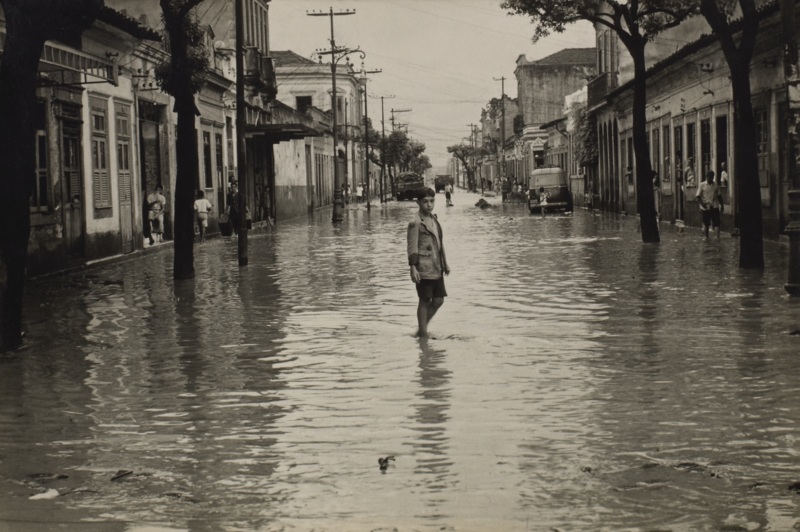
\includegraphics[width=\textwidth]{./images/PNLD0001-04.png}
\end{figure}

A apresentação das principais características do gênero crônica também
pode acontecer nesse momento. O tipo de narrador, o tema, o espaço/tempo
da narrativa, o desenvolvimento do texto, a intencionalidade,
ficção/realidade. É imprescindível a discussão sobre o veículo a partir
do qual a crônica circulava --- o jornal.

A leitura pode ser expandida para problemas que não estão
necessariamente expostos no texto, como os maus tratos aos animais,
abandonos, a maneira como os poderes públicos se posicionam a respeito.
Alunas e alunos podem trazer suas experiências a esse respeito.

Outro ponto relevante a ser explorado pode ser a supervalorização dos
\emph{pets}, fenômeno mais ou menos recente em nossa sociedade. A
quantidade imensa de lojas e serviços especializados em \emph{pets},
incluindo \emph{spas} e hotéis, mostra a maneira como o capitalismo se
apropriou e expandiu seu domínio sobre as relações afetivas entre seres
humanos e animais.

{\paragraph{Pós"-Leitura}}

Espera"-se que os alunos e alunas assimilem as questões básicas que
envolvem a escrita de uma crônica: a narrativa leve, que tem por
objetivo estabelecer um tipo de relação ``próxima'' como os leitores e
leitoras; um tema do cotidiano, o posicionamento do autor a respeito do
tema, que pode ser de crítica, afeto, compreensão, constatação ou
simplesmente a socialização de uma impressão ou uma ideia suscitada num
dado momento do cotidiano. Para tanto, a professora ou o professor pode
realizar atividades escritas e orais ou avaliações, com o objetivo de
aferir o desempenho dos alunos e alunas em relação à leitura e
compreensão da crônica. 


\begin{comment}
\begin{comment}

\subsubsection{\textit{As enchentes}}

\paragraph{\textit{Pré"-leitura}}

As alunas e alunos podem realizar pesquisas sobre enchentes,
deslizamentos de terra, desmoronamento de casas, que acontecem todos os
anos, no verão, quase sempre com vítimas fatais. Poderia ser pedida uma
atividade de pesquisa e socialização de histórias sobre enchentes ou
situações vividas por familiares, amigos ou até casos vivenciados pelos
próprios estudantes ou suas famílias.

\paragraph{\textit{Leitura}}

Aqui podem ser trabalhadas algumas questões relativas ao tipo de
escrita jornalística: a brevidade do texto, próximo da \emph{notícia}, a
linguagem objetiva e direta, centrada no referencial, o ponto de vista
do escritor, o desenvolvimento do tema, etc. Importante também que os
professores e professoras chamem atenção para a dimensão histórica de um
problema meteorológico, que tem consequências sociais gravíssimas e que
até hoje não foi enfrentado seriamente pelas autoridades. Esse texto é
um bom exemplo de uma crônica jornalística. Não era nada normal um
escritor do gabarito de Lima Barreto tratar de assuntos como esse. Tal
fato mostra que o autor estava preocupado com as catástrofes que
poderiam ser evitadas, se os responsáveis pela gestão pública se
preocupassem realmente com a vida das populações mais vulneráveis. Essa
crônica também possibilita uma aproximação com textos hoje em dia
veiculados em redes sociais, como posts no Facebook, por exemplo.

\paragraph{\textit{Pós"-leitura}}

Uma atividade interessante que pode ser despertada a partir da leitura
dessa crônica seria um tipo de fórum ou assembleia para discussão do
tema ``Enchentes'', o que envolveria outras áreas do conhecimento, como
Geografia, Sociologia. Questões relativas ao planejamento urbano,
ocupação de áreas vulneráveis, como encostas de morros e áreas de
várzea. Discutir maneiras e métodos de prevenção.

As alunas e alunos podem fazer o exercício de procurar outras fontes
textuais que tragam o mesmo problema: programas televisivos, matérias
jornalísticas (tanto da imprensa escrita, como audiovisual), sites,
blogs. O importante ao final da atividade é que as alunas e alunos
assimilem mais esse aspecto das crônicas de Lima Barreto, próxima
daquilo que hoje em dia conhecemos como artigo jornalístico, voltado
para problemas do cotidiano. De uma forma geral, no trabalho com as
crônicas, é importante que alunos e alunas assimilem a maneira pela qual
o escritor observou o evento cotidiano e deu um tratamento literário a
ele. Nesse processo, a escrita ganha emoções, sentimentos e afetos
experimentados pelo observador, sempre com linguagem simples e objetiva.

\paragraph{Tempo estimado} Duas a três aulas de 50 minutos para cada
crônica.

%\begin{enumerate}
%\def\labelenumi{\arabic{enumi})}
%\item
  %\begin{quote}
  %\textit{Tema: A linguagem e seus diferentes contextos e variações}
  %\end{quote}
%\end{enumerate}


%\begin{quote}
%\textit{(Habilidades BNCC: EM13LGG401, EM13LGG402, EM13LP45, EM13LP47 e EM13LP48)}
%\end{quote}

\marginnote{\footnotesize\textbf{EM13LGG402}\\
Analisar obras significativas da literatura brasileira e da literatura de outros países e povos, em especial a portuguesa, a indígena, a africana e a latino"-americana, com base em ferramentas da crítica literária (estrutura da composição, estilo, aspectos discursivos), considerando o contexto de produção (visões de mundo, diálogos com outros textos, inserções em movimentos estéticos e culturais etc.) e o modo como elas dialogam com o presente.\\\medskip
\textbf{EM13LP45}\\
Compartilhar sentidos construídos na leitura/escuta de textos literários, percebendo diferenças e eventuais tensões entre as formas pessoais e coletivas de apreensão desses textos, para exercitar o diálogo cultural e aguçar a perspectiva crítica.}


%Tema:
\subsection{A linguagem e seus diferentes contextos e variações}


\paragraph{Conteúdo} Esta atividade tem como base as cônicas
{\textit{Coisas do jogo do ``Bicho''}} e {\textit{Coisas de
``mafuá''}}. A ideia é apresentar e trabalhar com os alunos e alunas o
uso que Lima Barreto fazia da chamada `linguagem coloquial', de modo a
ampliar no texto o sentido de realidade, mas sem cair no pitoresco ou
encarar os dialetos como formas ``menores'' ou ``rudimentares'' de
expressão. Professores e professoras podem inserir na atividade a
questão da variação linguística, dos diversos contextos comunicacionais
em que a linguagem se desdobra em múltiplas possibilidades de uso.

\paragraph{Objetivos} Apresentar e trabalhar junto aos alunos e alunas as
possibilidades artísticas de se manejar a variação linguística. Mostrar
que existem contextos e situações comunicacionais que cobram
performances comunicativas específicas. As artes, em especial a
Literatura, o Teatro, a Música, o Cinema e as linguagens Audiovisuais de
uma forma geral são uma boa porta de entrada para a discussão sobre as
variações linguísticas.

\marginnote{\footnotesize\textbf{EM13LP47}\\
Analisar assimilações e rupturas no processo de constituição da literatura brasileira e ao longo de sua trajetória, por meio da leitura e análise de obras fundamentais do cânone ocidental, em especial da literatura portuguesa, para perceber a historicidade de matrizes e procedimentos estéticos.}

\paragraph{Justificativa} O fenômeno da variação linguística está muito
ligado à literatura e suas diversas modalidades. Hoje em dia, as regras
para a criação artística não se apresentam tão inflexíveis quanto foram
no passado. Quando lemos a prosa de Guimarães Rosa, Osman Lins, um livro
como ``Cidade de Deus'', de Paulo Lins, ou os livros dos escritores e
escritoras da literatura marginal, devemos ter em mente que um dos
batalhadores para que esse tipo de linguagem ganhasse uma estatura
artística ampliada foi justamente Lima Barreto. Foi um escritor muito
criticado por seu aparente ``desleixo'' no uso da linguagem, pois
escreveu numa época em que a normatividade da língua portuguesa era
imposta quase de forma inconteste.

\paragraph{Metodologia} A leitura e compreensão dos textos são
fundamentais para o bom desempenho dessa atividade. Uma leitura feita em
sala de aula, de forma coletiva, com o professor ou professora já
apropriados da narrativa, pode ser um bom caminho. Alguns procedimentos
que podem auxiliar no entendimento geral do texto são os seguintes:

%\begin{enumerate}
%\def\labelenumi{\arabic{enumi})}
%\item
  %Para a crônica {\textit{Coisas do jogo do ``Bicho''}}
%\end{enumerate}

\begin{figure}[ht!]
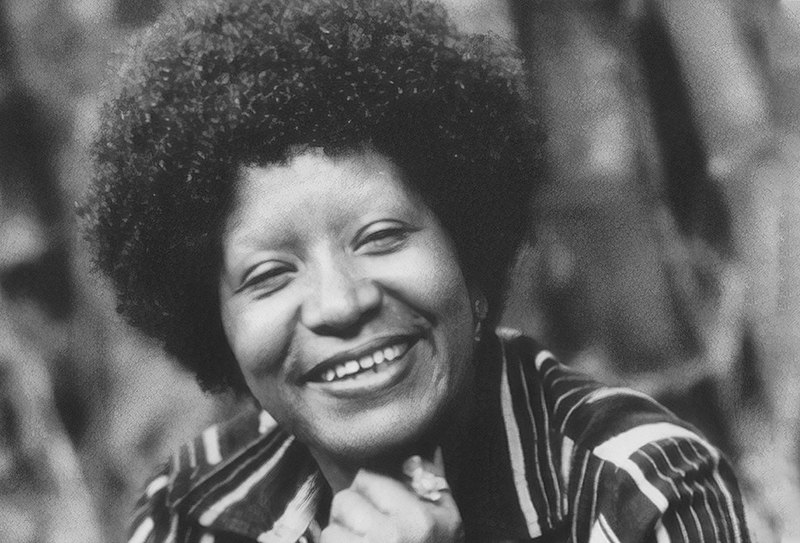
\includegraphics[width=\textwidth]{./images/PNLD0001-05.png}
\end{figure}

\subsubsection{\textit{Coisas do jogo do ``Bicho''}}

\paragraph{\textit{Pré"-leitura}}

O educador ou a educadora pode perguntar para a turma se conhecem o
jogo do bicho. Muitos provavelmente vão dizer que sim. Se algum
voluntário quiser, e souber, pode explicar como funciona o jogo. É uma
maneira de aproximar os alunos e alunas da temática do texto. A
pré"-leitura pode ser expandida para uma pequena pesquisa histórica,
feita pelo professor ou professora, ou mesmo solicitada como atividade
para os alunos e alunas. Como se trata de um assunto controverso, pois o
jogo do bicho é um tipo de loteria ``extra"-oficial'' e implica em
sansões penais, inclusive, a contextualização é um pressuposto
importante.

\paragraph{\textit{Leitura}}

A parte que interessa mais diretamente à atividade é a ``carta'' que um
apostador do jogo do bicho endereçou ao personagem Bico"-Doce, do jornal
\emph{Talismã}. É importante que no processo de leitura os alunos e
alunas percebam os ``erros'' contidos no texto. Uma nota de rodapé
contida na crônica apresenta esse procedimento como sendo um traço
estilístico do texto. Algumas questões que podem ser levantadas após a
leitura e compreensão do texto:

Por que o autor escreveu a ``carta'' de modo a apresentá"-la com os
erros de ortografia e escrita? Quais objetivos estéticos ele vislumbrou?
O que mudaria no texto se a ``carta'' endereçada ao senhor Bico"-Doce
tivesse sido escrita em conformidade com os padrões normativos da língua
portuguesa?

A qual contexto social o traço estilístico presente na ``carta''
remete o leitor ou a leitora? Quais problemas ele aponta?

Com apoio de bibliografia extra, o professor ou a professora pode
aprofundar essa discussão. Um bom livro para essa temática é o
``Preconceito linguístico'', do professor Marcos Bagno, ou os escritos
de Lélia Gonzales, sobre o ``pretuguês'', que podem ser acessados
através do link:
\url{https://outraspalavras.net/eurocentrismoemxeque/para"-compreender"-a"-amefrica"-e"-o"-pretugues/}

\paragraph{\textit{Pós"-leitura}}

Como atividade de fixação e treino da escrita normativa, o professor ou
a professora pode solicitar aos alunos e alunas para ``reescreverem'' a
carta endereçada ao senhor Bico Doce, mas de forma a ``corrigir'' os
erros e deixar o texto em uma linguagem que obedeça às normas e regras
gramaticais da Língua Portuguesa.

Outra ideia seria escrever a carta com a linguagem coloquial e gírias
usadas pelos e pelas estudantes ou o tipo de linguagem utilizada para
troca de mensagens nas redes sociais. Qual seria seu estilo, sua maneira
de escrever coloquialmente esta carta? Podem brincar com a linguagem da
internet com as abreviações, usar termos de outros partes do país, de
outros estados.

\begin{figure}[ht!]
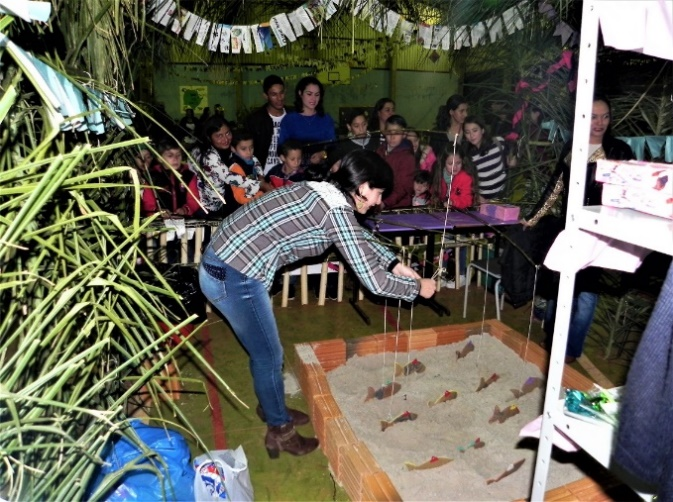
\includegraphics[width=\textwidth]{./images/PNLD0001-06.png}
\end{figure}

\subsubsection{\textit{Coisas de ``mafuá''}}

\paragraph{\textit{Pré"-leitura}}

Na seção ``Cotidiano e Vida nos Subúrbios'' existem quatro crônicas que
apresentam o tema do ``mafuá''. Se o professor ou a professora desejarem
realizar uma atividade em profundidade sobre o tema, a sugestão é que
realizem junto aos alunos e alunas um trabalho de leitura de todos os
textos. Alguns apontamentos que poder ser aprofundados se este caminho
for seguido:

\marginnote{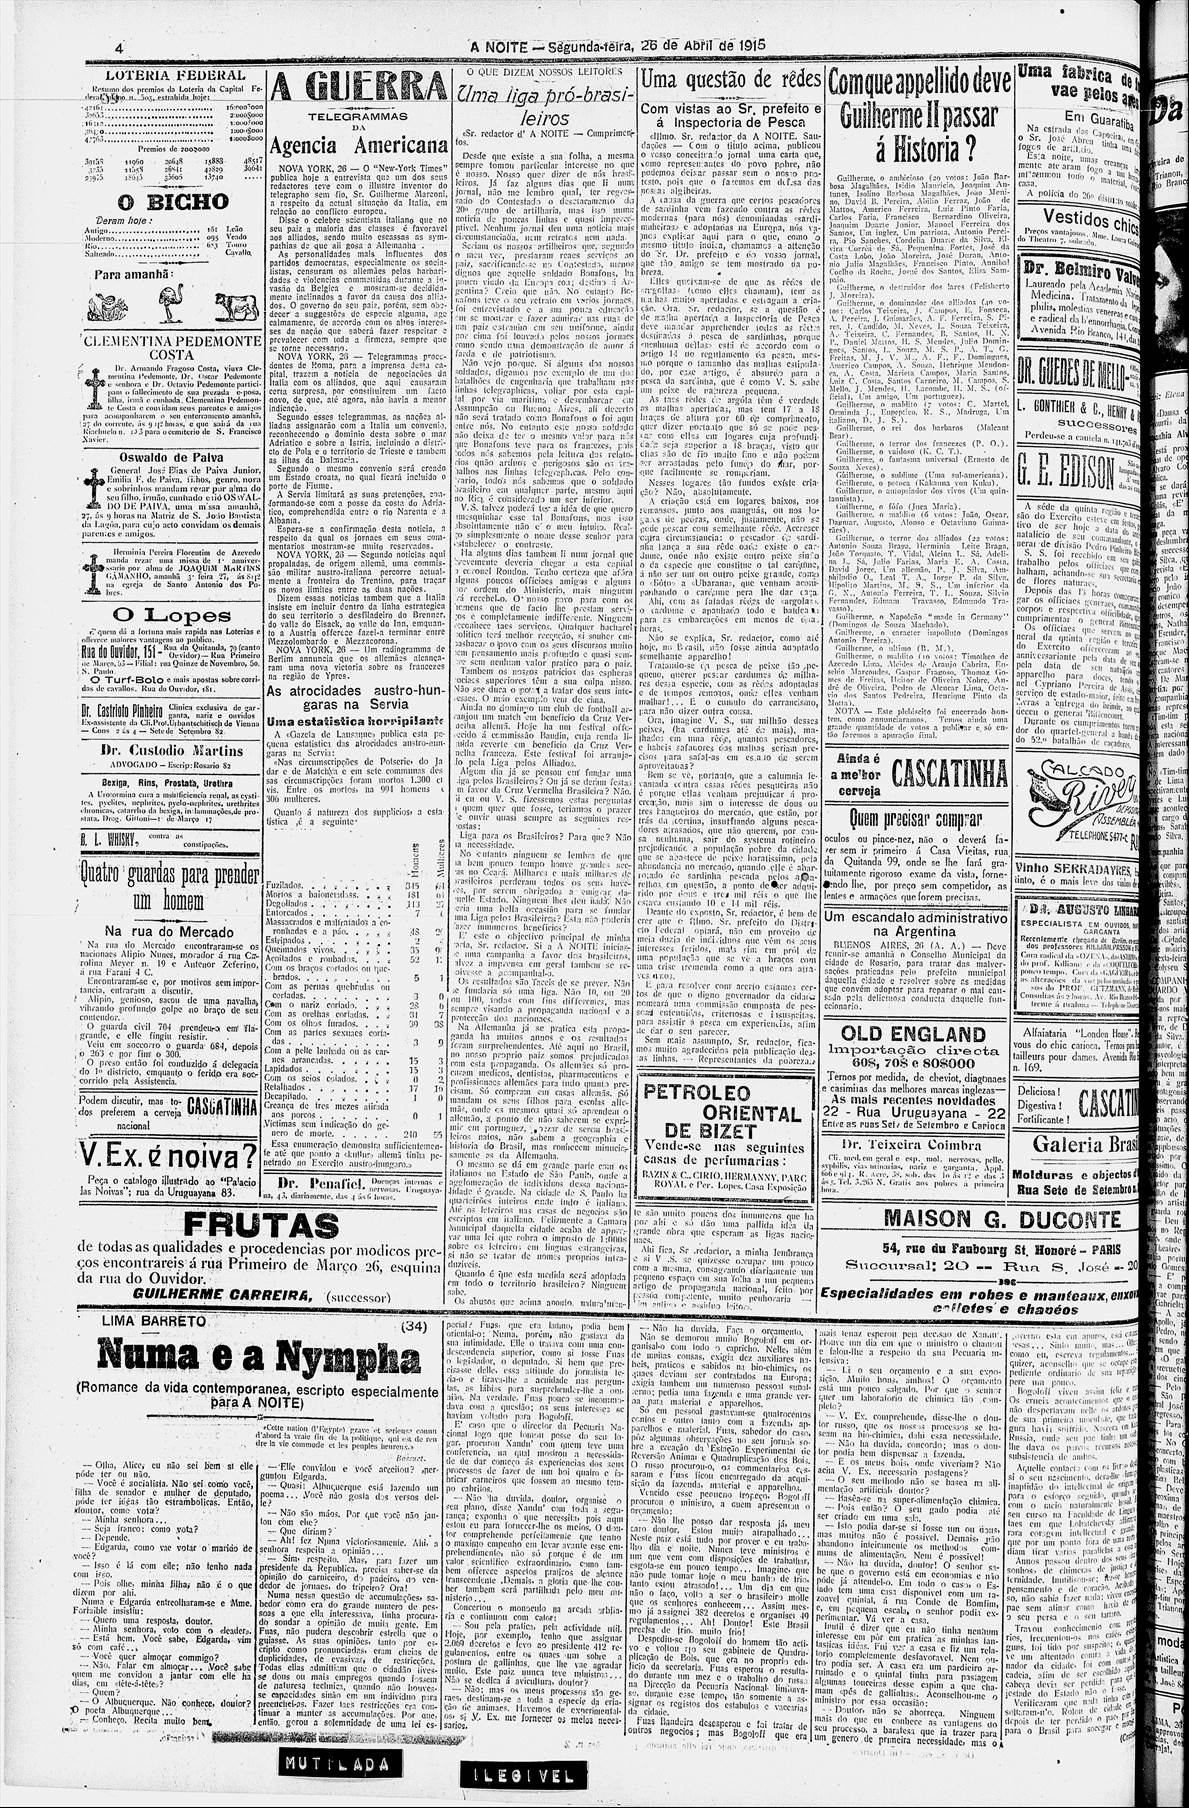
\includegraphics[width=5cm]{./images/PNLD0001-07.png}\\
\textit{Foto do autor}}

As alunas e alunos podem compreender a diferença entre a crônica
{\textit{Feiras e ``mafuás''}} e \textit{\emph{No ``mafuá'' dos
padres}} em relação às outras duas crônicas, que têm um desenvolvimento
mais inclinado à ficção ou à crônica literária. Nos dois primeiros
textos, a escrita é mais próxima da objetividade jornalística,
principalmente em {\textit{Feiras e ``mafuás''}}, que apresenta um
desenvolvimento mais próximo de um artigo ou pequeno ensaio sociológico,
histórico e antropológico, além de tratar de questões históricas, como o
advento da República, o positivismo, etc. Mas o que nos interessa mais
de perto para esta atividade é a existência de um empenho didático por
parte do escritor em apresentar o ``\emph{mafuá}'' para aqueles que não
o conhecem e para isso a linguagem é objetiva, referencial.

Depois da leitura de \textit{\emph{Feiras e ``mafuás''}} e
{\textit{No ``mafuá'' dos padres}}, o professor ou professora podem
discutir alguns pontos. Por exemplo: perguntar aos alunos e alunas sobre
as ``quermesses'' que acontecem durante o período das festas juninas,
pois existem muitas semelhanças entre os dois eventos. Uma pergunta
disparadora seria: As ``quermesses'' não seriam uma forma de
``\emph{mafuá}''? Quais são as ``prendas'' existentes nas barraquinhas
das ``quermesses'' que acontecem em nossa época?

Pode"-se também buscar por outras referências que aprofundem o
entendimento desse tipo de acontecimento e diversão e seu relacionamento
com as festas juninas. Suas origens, significados.

\paragraph{\textit{Leitura}}

\marginnote{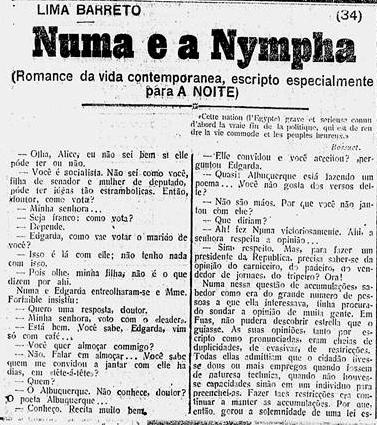
\includegraphics[width=5cm]{./images/PNLD0001-08.png}\\
\textit{Foto do autor}}

Para o trabalho centrado na crônica {\textit{Coisas de ``mafuá''}},
dentro dos objetivos mais específicos dessa atividade --- apresentação e
compreensão do fenômeno da variação linguística --- o procedimento
metodológico continua o mesmo: leitura e compreensão do texto de uma
maneira geral, comentários, impressões, etc. Em termos de composição, a
crônica {\textit{Coisas de ``mafuá''}} é muito próxima de
{\textit{Paulino e o ``mafuá''}}. Ambas se constituem de um ``texto
dialogado'', com linguagem simples, desenvolvimento curto e um tom de
humor. No entanto, em {\textit{Coisas de ``mafuá''}} existe algo de
específico em relação às demais. Trata"-se do uso de gírias, tais como
``xadrez'', ``cobres'', ``algum'', ``canoa'', ``lelé''. Esse é o ponto
que esperamos que seja explorado ao longo da leitura.

Hoje em dia não nos espanta que um escritor ou escritora faça uso de
gírias e linguagem coloquial em textos literários. Mas, na época em que
Lima Barreto escreveu esse texto tal procedimento era bastante inovador
e desafiador. Mais do que isso, conforme já foi demonstrado na atividade
com a crônica {\textit{Coisas do jogo do ``Bicho''}}, o uso da
linguagem coloquial está diluído no próprio corpo do texto, com bastante
naturalidade e sem que o autor queira demonstrar que se trata de algo
exótico.

A única marca individualizadora para as gírias são as aspas, que o
escritor utiliza para chamar atenção do público leitor, que muito
provavelmente não estava familiarizado com tais expressões. Essa
contextualização da época da escrita e do caráter inovador da prosa de
Lima Barreto é de suma importância para os objetivos desta atividade.

\paragraph{\textit{Pós"-leitura}}

Pedir para que alunas e alunos façam, após leitura e compreensão do
texto, um levantamento das palavras que aparecem entre aspas. Num
segundo momento, a atividade pode ser direcionada para a significação
das gírias. Por exemplo: ``xadrez'' (prisão, cadeia), ``canoa'' (viatura
da polícia), ``lelé'' (escarcéu, confusão).

Outra atividade pode ser a solicitação de trabalhos individuais ou em
grupos, com pesquisas de termos específicos ou gírias contemporâneas.
Podem servir como material de pesquisa: músicas, filmes, canais de
youtube, jogos, modalidades esportivas, etc. Como referência, pode"-se
partir de série de vídeos do youtuber Charles Santos sobre as gírias do
estilo musical contemporâneo \emph{Trap}\footnote{Disponível no link:
  \url{https://www.youtube.com/watch?v=ZDB79gIitU0}}:

Uma pesquisa com pessoas mais velhas da família ou conhecidos pode ser
uma boa atividade para recolher gírias antigas ou expressões que não são
mais utilizados atualmente.

\paragraph{Tempo estimado} Duas a três aulas de 50 minutos para cada
crônica.

%\begin{enumerate}
%\def\labelenumi{\arabic{enumi})}
%\item
  %\begin{quote}
  %\textit{Tema: Clube da crônica e laboratório de criação}
  %\end{quote}
%\end{enumerate}

%\begin{quote}
%\textit{(Habilidades BNCC: EM13LGG301, EM13LGG703, EM13LGG704, EM13LP27,
%EM13LP29, EM13LP46, EM13LP50 e EM13LP53)}
%\end{quote}

%\paragraph{Tema:}

\subsection{Clube da crônica e laboratório de criação}

\marginnote{\footnotesize\textbf{EM13LGG703}\\
Utilizar diferentes linguagens, mídias e ferramentas digitais em processos de produção coletiva, colaborativa e projetos autorais em ambientes digitais.\\\medskip
\textbf{EM13LGG704}\\
Apropriar-se criticamente de processos de pesquisa e busca de informação, por meio de ferramentas e dos novos formatos de produção e distribuição do conhecimento na cultura de rede.\\\medskip
\textbf{EM13LP27}\\
Organizar situações de estudo e utilizar procedimentos e estratégias de leitura adequados aos objetivos e à natureza do conhecimento em questão. Competências específicas: 3, 7\\\medskip
\textbf{EM13LP29}\\
Realizar pesquisas de diferentes tipos (bibliográfica, de campo, experimento científico, levantamento de dados etc.), usando fontes abertas e confiáveis, registrando o processo e comunicando os resultados, tendo em vista os objetivos colocados e demais elementos do contexto de produção, como forma de compreender como o conhecimento científico é produzido e apropriar-se dos procedimentos e dos gêneros textuais envolvidos na realização de pesquisas.\\\medskip
\textbf{EM13LP50}\\
Selecionar obras do repertório artístico-literário contemporâneo à disposição segundo suas predileções, de modo a constituir um acervo pessoal e dele se apropriar para se inserir e intervir com autonomia e criticidade no meio cultural.}


\paragraph{Conteúdo} Criação de grupos de estudo e laboratórios de criação
textual/literária a partir do gênero crônica. A formação dos grupos pode
obedecer a diversos critérios --- interesse por temas presentes na
\emph{Antologia}, interesse por outras áreas do conhecimento (História,
Sociologia, Filosofia, Geografia, Jornalismo). Os grupos também podem
contar com alunos e alunas de diferentes séries do Ensino Médio ou de
salas diferentes de uma mesma série. Professoras e professoras
participam como coordenadores/estimuladores, na estruturação inicial dos
grupos, ajudam na curadoria de outros escritores e escritoras, na
articulação com outros professores e professoras de outras áreas do
conhecimento, na disponibilização de lugares para os encontros --
bibliotecas, salas de pesquisa, acesso a computadores.

\paragraph{Objetivos} Promover um trabalho de longo prazo, com
protagonismo dos e das estudantes do Ensino Médio, tendo como eixo
estruturante a linguagem literária. Estimular a leitura, pesquisa,
discussão, socialização, produção e publicação de textos próprios ou de
escritores e escritoras, não somente brasileiros(as), que praticaram e
praticam o gênero crônica. Estimular o trabalho coletivo, a iniciação à
pesquisa, curadoria e a autonomia intelectual dos e das estudantes do
Ensino Médio.

\paragraph{Justificativa} De acordo com as diretrizes estipuladas pela
\textsc{bncc} para a criação de atividades que promovam a articulação entre áreas
do conhecimento, os \textit{Grupos} se constituem como
\emph{agrupamentos de estudantes livremente associados que partilham de
gostos e opiniões comuns (leitura, conservação ambiental, desportivo,
cineclube, fã"-clube, fandom etc.)}. Por sua vez, os
\textit{Laboratórios} \emph{supõem atividades que envolvem observação,
experimentação e produção em uma área de estudo e/ou o desenvolvimento
de práticas de um determinado campo (línguas, jornalismo, comunicação e
mídia, humanidades, ciências da natureza, matemática etc.}

A partir da criação e promoção do trabalho em grupos e do
desenvolvimento de laboratórios, os alunos e alunas têm a possibilidade
de desenvolver autonomia e proatividade em diversas esferas de
organização, além dos objetivos mais específicos buscados pela
atividade, que consistem na prática sistemática de leitura, pesquisa e
escrita de textos, tendo como base o gênero crônica.

\paragraph{Metodologia} A primeira parte do projeto consiste na
estruturação básica dos grupos, através da divulgação das atividades,
que podem acontecer em sala de aula ou em pontos da escola destinados a
colocação de avisos, cursos e informes gerais.

As atividades iniciais podem seguir a metodologia explorada nas
Propostas de Atividade 1 e 2 deste manual. Outros escritores e
escritoras, tanto apresentados pelos educadores ou educadoras, ou por
alunos e alunas, podem começar a compor uma ``biblioteca de crônicas''.
Um segundo momento de ampliação do repertório de cronistas acontece
através de pesquisas, realizadas no próprio acervo da escola, em
bibliotecas públicas ou pela internet. A seleção das crônicas a serem
lidas e compartilhadas obedecerá a critérios estabelecidos pelos
próprios grupos ou coletivos.

As atividades poder ser organizadas por eixos de trabalho, tais como: 1)
Períodos de encontro para leitura; 2) Períodos de encontro para
discussão das leituras; 3) Pesquisas; 4) Encontros de apresentação de
pesquisas (novos autores e autoras, obras, seleção de crônicas etc.)

Os \textit{Laboratórios} se constituem como uma etapa posterior e podem
ser organizados pelos próprios estudantes a partir de um eixo comum. Por
exemplo: 1) Criação de \emph{blogs}, perfis no Instagram, canais no
Youtube ou \emph{websites} para publicação de crônicas. 2) Organização
de oficinas de produção textual, tendo como base o gênero crônica. Aqui
podem ser elaboradas técnicas de edição simples, como \emph{zines},
jornais, revistas, o que possibilita, também, uma intersecção entre
texto e linguagens visuais. 3) Organização de encontros literários ou
rodas de leitura/apresentação, tais como acontecem nos \emph{\textsc{slams}} e
saraus. 4) Bate papos com escritoras escritores e convidados, que podem
ser também em formato de \emph{lives}.

\paragraph{Tempo estimado} Um semestre.

%\begin{enumerate}
%\def\labelenumi{\arabic{enumi})}
%\item
  %\begin{quote}
  %\textit{Tema: Aprendendo sobre o Conto como gênero literário.}
  %\end{quote}
%\end{enumerate}

%\begin{quote}
%\textit{(Habilidades BNCC EM13LGG703; EM13LGG704; EM13LP16; EM13LP36 e EM13LP44)}
%\end{quote}

%\paragraph{Tema:}
\subsection{Aprendendo sobre o Conto como gênero literário}

\marginnote{\footnotesize\textbf{EM13LGG703}\\
Utilizar diferentes linguagens, mídias e ferramentas digitais em processos de produção coletiva, colaborativa e projetos autorais em ambientes digitais.\\\medskip
\textbf{EM13LGG704}\\
Apropriar-se criticamente de processos de pesquisa e busca de informação, por meio de ferramentas e dos novos formatos de produção e distribuição do conhecimento na cultura de rede.}

\paragraph{Conteúdo} A partir dos contos \textit{\emph{A cartomante}} e
{\textit{O homem que sabia javanês}}, elaborar estratégias e
processos de leitura que apresentem o gênero literário ``conto'' em suas
dimensões históricas e estéticas. Especificar as diferenças e
convergências entre os gêneros ``conto'' e ``crônica'', principalmente
para se compreender a forma como esses gêneros aparecem na literatura
contemporânea, em que a fronteiras entre um e outro não são mais tão
rígidas quanto eram na época em que Lima Barreto produziu sua obra.

\paragraph{Objetivos} Trabalhar, junto aos alunos e alunas do Ensino
Médio, as especificidades do gênero conto. Ao lado da crônica, o conto
se constitui como uma boa porta de entrada para se estimular a leitura
de obras literárias, praticar interpretações, compreender os componentes
formais que possibilitam a composição literária, tais como personagens,
foco narrativo, enredo, temática, narrador, temporalidade e
espacialidade da narrativa, entre outros.

\marginnote{\footnotesize\textbf{EM13LP16}\\
Utilizar softwares de edição de textos, fotos, vídeos e áudio, além de ferramentas e ambientes colaborativos para criar textos e produções multissemióticas com finalidades diversas, explorando os recursos e efeitos disponíveis e apropriando-se de práticas colaborativas de escrita, de construção coletiva do conhecimento e de desenvolvimento de projetos. Competências específicas: 7\\\medskip
\textbf{EM13LP36}\\
Conhecer e analisar diferentes projetos editorias – institucionais, privados, públicos, financiados, independentes etc. –, de forma a ampliar o repertório de escolhas possíveis de fontes de informação e opinião, reconhecendo o papel da mídia plural para a consolidação da democracia. Competências específicas: 2 \\\medskip
\textbf{EM13LP44}\\
Analisar, discutir, produzir e socializar, tendo em vista temas e acontecimentos de interesse local ou global, notícias, fotodenúncias, fotorreportagens, reportagens multimidiáticas, documentários, infográficos, podcasts noticiosos, artigos de opinião, críticas da mídia, vlogs de opinião, textos de apresentação e apreciação de produções culturais (resenhas, ensaios etc.) e outros gêneros próprios das formas de expressão das culturas juvenis (vlogs e podcasts culturais, gameplay etc.), em várias mídias, vivenciando de forma significativa o papel de repórter, analista, crítico, editorialista ou articulista, leitor, vlogueiro e booktuber, entre outros. Competências específicas: 1, 3}

\paragraph{Justificativa} A \emph{Antologia de crônicas e contos de Lima
Barreto} foi pensada tanto para que os textos sejam trabalhados em sua
individualidade, quanto numa perspectiva de conjunto. No caso dos
contos, que só aparentemente se constitui como uma narrativa ``fácil'',
a disposição dos textos obedece a uma intenção didática: possibilitar a
fruição e compreensão do gênero a partir de suas formulações mais
simples --- o que já aparece na seção ``Humor'' --- e caminhar para
composições mais complexas. Por se tratar de uma das mais antigas formas
literárias, e pela multiplicidade de feições que esse gênero pode adotar
--- conto fantástico, conto de terror, conto realista, conto dialogado,
conto de fadas, psicológico, popular; hoje em dia ainda temos o
``miniconto'' e o ``microconto'', muito praticado em redes sociais como
o Twitter --- essa narrativa breve, muitas vezes de fácil compreensão,
esconde uma técnica de escrita bastante apurada.

\paragraph{Metodologia} Qualquer um dos dois contos selecionados para esta
atividade pode ser trabalhado em sala de aula de modo a introduzir o
gênero e desenvolver as competências e habilidades mínimas para a
leitura de outros e outras contistas. A seguir algumas propostas que
podem ser desenvolvidas no processo de leitura.

%\begin{enumerate}
%\def\labelenumi{\arabic{enumi})}
%\item
  %Para o conto \textit{\emph{A cartomante}:}
%\end{enumerate}

\subsubsection{\textit{A cartomante}}

\paragraph{\textit{Pré"-leitura}}

Este será o primeiro contato de análise e interpretação por parte das
alunas e alunos com os contos escritos por Lima Barreto que constam na
\emph{Antologia}. Se o professor ou professora já realizou algum
trabalho com as crônicas presentes no livro, a retomada das
características técnicas presentes naqueles textos pode ser uma boa
atividade para se iniciar a leitura do conto. Outra possibilidade
consiste em assistir a série de vídeos produzidos pelo canal ``Brasil
Escola'' dedicados ao gênero conto.\footnote{Para acessar o primeiro dos
  vídeos, seguir o link:
  \url{https://www.youtube.com/watch?v=c"-rge5nGRyk}}

\paragraph{\textit{Leitura}}

Importante salientar junto aos alunos e alunas que este texto está
presente na primeira parte da \emph{Antologia}, que é destinada às
crônicas. Isso se deve ao fato de Lima Barreto ter estabelecido um tipo
de narrativa híbrida, um texto que é meio conto, meio crônica. Hoje em
dia, \textit{\emph{A cartomante}} pode tranquilamente figurar como um
conto, mas na época de sua escrita estava mais para uma crônica
literária --- aquela que traz aspectos do cotidiano, mas com um
desenvolvimento mais acentuado à prosa de ficção. Essa narrativa, bem
como as demais presentes na seção ``Humor'', mostram como os gêneros
literários sofrem mudanças em sua concepção ao longo do tempo.

A leitura pode ser realizada individual ou coletivamente. Em sala de
aula, após a leitura, a professora ou o professor pode discutir com os
alunos alguns tópicos de entendimento do texto, por exemplo: 1)O tipo de
narrador (em terceira pessoa); 2) Quais personagens aparecem (o marido,
a esposa, o cunhado, as filhas, a ``cartomante''); 3) Qual o conflito
que proporciona e alimenta o desenvolvimento da narrativa (as
dificuldades financeiras do ``chefe de família'', a crença em alguma
``mandinga'', provavelmente encomendada pelo cunhado); 4) As dimensões
de tempo/espaço (a esfera doméstica / a esfera pública no Rio de
Janeiro, início do século \textsc{xx}); 5) O clímax (desenlace do conflito).

Uma vez realizada a leitura mais técnica da narrativa, a atividade
interpretativa pode caminhar para camadas mais profundas do texto. Por
exemplo: 1) a estrutura da família patriarcal, que cobra do homem a
responsabilidade pelo sustento da casa; 2) o papel ``secundário'' que a
mulher ocupa, num plano mais superficial do texto, mas que na verdade é
ela quem está sustentando toda aquela situação, trabalhando como
lavadeira (em casa) e cartomante (na rua), ou seja, em dupla jornada, ou
tripla; 3) o preconceito em relação às formas de religiosidade de matriz
africana, que opera também como pano de fundo no conto, na desconfiança
do marido de que aquela situação tinha por causa alguma ``coisa feita'',
realizada por algum ``preto mina'', sob encomenda do próprio Cunhado; 4)
a situação de desespero ocasionada pelo desemprego, fato que levou,
neste caso, o marido a supor que a vida não ia para frente por conta de
``forças ocultas'' e não pela situação econômica do país.

A partir deste trabalho prévio de leitura e interpretação, tanto das
técnicas de composição quanto dos temas que aparecem no texto, o
professor ou a professora pode analisar aquilo que seria o cerne do
gênero conto: a brevidade. Tal conceito é fundamental para que o conto
``funcione'' como narrativa que instaura um processo de reflexão
imediatamente ao final de sua leitura. No texto {\textit{A
cartomante,}} Lima Barreto utiliza a técnica da surpresa ou do ``final
revelador'', mais especificamente, um \emph{anticlímax}, que subverte as
expectativas que os leitores e leitoras vão construindo ao longo da
narrativa. E tudo isso em apenas duas páginas.

\paragraph{\textit{Pós"-leitura}}

O professor ou a professora pode discutir junto aos alunos e alunas a
possibilidade de, com uma estrutura temática tão profunda quanto a que
encontramos em {\textit{A cartomante}}, o escritor poder conseguir
transformar essa pequena narrativa em um romance de maior fôlego. Nesse
sentido, a \emph{Antologia} apresenta dois contos de Lima Barreto que
sofreram esse processo de ampliação. São eles {\textit{Clara dos
Anjos}} e {\textit{Numa e a Ninfa}}. Inicialmente escritos no
gênero conto, esses dois textos ganharam desenvolvimento e se
transformaram em romances, cujos nomes continuaram os mesmos de suas
respectivas formulações originais. O romance ``Numa e a Ninfa'' foi
publicado em folhetins no jornal \emph{A noite} e depois editado em
livro no ano de 1915. \emph{Clara dos Anjos}, romance, foi publicado
postumamente em capítulos, pela revista \emph{Souza Cruz}, durante o ano
de 1924. Somente em 1948 a obra ganhou sua edição em livro, pela editora
Mérito S.A.

Algumas atividades podem ser requisitadas para que os professores e
professoras avaliem o nível de entendimento dos alunos acerca do gênero
conto. Um caminho interessante seria uma atividade interpretativa,
realizada pelos alunos e alunas, individualmente ou em grupos, de outro
conto presente na \emph{Antologia} e que tenha características
semelhantes, por exemplo: {\textit{O Gambá}}, {\textit{A
barganha}}, {\textit{Milagre do Natal}} e {\textit{Quase ela
deu o ``sim''}}.

%2) Para o conto {\textit{O homem que sabia javanês}}
\subsubsection{\textit{O homem que sabia javanês}}

Esse é um dos mais famosos contos da literatura brasileira. Existem,
inclusive, algumas adaptações dessa pequena obra prima de nossas letras
para outras formas de linguagem. Destacamos uma adaptação de
{\textit{O homem que sabia javanês}} em quadrinhos, lançada pela
Editora Itapuca, dentro da coleção \emph{Literatura brasileira em
quadrinhos}. Além do filme --- média"-metragem --- ``O Homem que sabia
javanês'', com direção e roteiro de Xavier de Oliveira, lançado em
2004\footnote{O filme pode ser acessado através desse link:
  \url{https://www.youtube.com/watch?v=DU9HxLRWPJ0\&t=190s}}. São
composições que podem ser utilizadas para atividades junto ao conto em
sua formatação original.

\paragraph{\textit{Pré"-leitura}}

Para as atividades de pré"-leitura do texto, podem ser retomadas e
discutidas com os alunos e alunas as mesmas premissas técnicas que
estipulamos para o trabalho em relação ao texto {\textit{A
cartomante}}, ou seja: 1) Leitura realizada individual ou coletivamente;
2) O tipo de narrador (um conto dialogado, narrado em primeira pessoa);
3) Personagens (Castelo, Castro, Barão de Jacuecanga, o Velho Preto
Africano, a dona Maria da Glória e seu Marido); 4) O conflito que
alicerça a narrativa (as dificuldades financeiras de Castelo que, apesar
de ser \emph{bacharel}, vivia de aplicar golpes); 5) As dimensões de
tempo/espaço (Rio de Janeiro, começo do século \textsc{xx}, os diferentes espaços
que alicerçam a história); 6) Clímax (desenlace do conflito).

Pode"-se, ainda como atividade preliminar, ser realizada uma sessão de
exibição do filme ``O homem que sabia javanês'' ou que os professores e
professoras indiquem o filme para que os alunos e alunas assistam antes
do início dos trabalhos com o texto.

\paragraph{\textit{Leitura}}

Assim como os demais textos de Lima Barreto, este conto apresenta uma
linguagem de época, com muitas palavras e expressões que não são de
amplo conhecimento. Embora o texto conte com muitas notas de rodapé,
ainda se faz necessária uma leitura mais atenta. É preciso sempre chamar
a atenção dos alunos e alunas para a importância de se buscar o
significado das palavras desconhecidas, com o uso de dicionários --
físicos ou ­\emph{on"-line}.

Um ponto importante para a compreensão desse conto consiste no
entendimento de sua estrutura narrativa. Torna"-se importante a
contextualização entre as nuances que envolvem o narrador (em primeira
pessoa) e o personagem Castelo. Embora seja um personagem"-narrador,
Castelo é também um ótimo contador de ``causos'' e essas três instâncias
se fundem no processo narrativo. O conto, em sua anatomia enunciativa,
funciona como uma rememoração, por parte do narrador"-personagem, de uma
conversa que teve, em uma confeitaria, com seu amigo Castro. Não é,
portanto, um conto ``100 por cento'' dialogado, se bem que os diálogos
funcionam como técnica fundamental para o desenvolvimento do texto.

Professores e professoras podem aprofundar essa questão do narrador, ou
foco narrativo, utilizando outros textos que apresentem outras técnicas
de composição narrativa. O narrador de \textit{\emph{O homem que sabia
javanês}} é o próprio Castelo, que funciona também como personagem
principal, contador de causos e aplicador de golpes. Sabemos que muitas
pessoas que vivem de aplicar golpes também gostam de contar suas
façanhas, daí a escolha feita por Lima Barreto, do ponto de vista da
técnica narrativa, ter sido bastante feliz. Um narrador em ``terceira
pessoa'' talvez não dotasse o texto de tanta força de realidade.

Tanto em {\textit{A cartomante}} quanto em \textit{\emph{O homem
que sabia javanês}} o escritor trabalha questões relativas à
subsistência, às maneiras através das quais os e as personagens buscam
ganhar dinheiro. Esse é um eixo temático que pode ser trabalhado com os
alunos e alunas. Quais as estratégias utilizadas pelos personagens para
driblar as dificuldades financeiras? Quais lugares sociais ocupam na
estrutura socioeconômica da sociedade? Que tipo de sociedade emerge e
alicerça as histórias? Importante destacar as diferenças entre os dois
contextos sociais internos às narrativas: em \textit{\emph{A
cartomante}} trata"-se de uma família pobre, quase sem os recursos
mínimos para a sobrevivência; já em \textit{\emph{O homem que sabia
javanês}} temos um personagem de classe média, bacharel, que se mostra
avesso ao trabalho continuado e assalariado.

\paragraph{\textit{Pós"-leitura}}

Um trabalho interessante seria a comparação entre o texto e a
adaptação para o cinema. Neste caso, alunas e alunos podem desenvolver
atividades de comparação entre as duas linguagens, construir uma
percepção imagética do período em que se passa a narrativa. O filme traz
uma construção cenográfica e de figurino que reproduz a ``cultura da
época''.

\paragraph{Tempo estimado} Duas a três aulas de 50 minutos para cada conto.

\section{Propostas de atividades 2}

%\begin{enumerate}
%\def\labelenumi{\arabic{enumi})}
%\item
  %\textit{Tema: Racismo, Futebol e Literatura}
%\end{enumerate}


%\textit{(Habilidades BNCC - EM13CHS501; EM13CHS502; EM13CHS503;
%EM13CHS504 e EM13CHS601)}

%\paragraph{Tema:}

\subsection{Racismo, Futebol e Literatura}

\marginnote{\footnotesize\textbf{EM13CHS501}\\
Compreender e analisar os fundamentos da ética em diferentes culturas, identificando processos que contribuem para a formação de sujeitos éticos que valorizem a liberdade, a autonomia e o poder de decisão (vontade). \\\medskip
\textbf{EM13CHS502}\\
Analisar situações da vida cotidiana (estilos de vida, valores, condutas etc.), desnaturalizando e problematizando formas de desigualdade e preconceito, e propor ações que promovam os Direitos Humanos, a solidariedade e o respeito às diferenças e às escolhas individuais. }

\paragraph{Conteúdo} A partir da crônica {\textit{Macaquitos}} e do
conto {\textit{O Pecado}}, a atividade consiste em trabalhar junto
aos alunos e alunas o complexo tema do racismo e do preconceito racial
no Brasil, sem perder o foco na Literatura. \emph{Considera"-se
importante, também, acrescentar junto à atividade algumas noções
relativas à preeminência que Lima Barreto, escritor afrodescendente,
concedeu ao problema da desigualdade racial e do preconceito de cor em
boa parte de sua obra.} O professor ou a professora pode trazer outras
narrativas de Lima Barreto, que não estão contempladas na
\emph{Antologia}, de modo a ampliar os recursos para a atividade.

\paragraph{Objetivos} A partir da leitura e análise dos textos literários
selecionados para a atividade, objetiva"-se construir junto aos alunos e
alunas um entendimento crítico sobre as manifestações que conhecemos
como racismo estrutural. Mostrar e analisar a maneira pela qual o autor
incorporou essas questões ao longo das narrativas. Estimular os alunos e
alunas a debaterem, de maneira crítica e conceitual, a persistência
desse fenômeno entre nós e a enxergarem seus fundamentos históricos,
econômicos, culturais que ainda se manifestam na atualidade.

\marginnote{\footnotesize\textbf{EM13CHS503}\\
Identificar diversas formas de violência (física, simbólica, psicológica etc.), suas causas, significados e usos políticos, sociais e culturais, avaliando e propondo mecanismos para combatê-las, com base em argumentos éticos.\\\medskip
\textbf{EM13CHS504}\\
Analisar e avaliar os impasses ético-políticos decorrentes das transformações científicas e tecnológicas no mundo contemporâneo e seus desdobramentos nas atitudes e nos valores de indivíduos, grupos sociais, sociedades e culturas.\\\medskip
\textbf{EM13CHS601}
Relacionar as demandas políticas, sociais e culturais de indígenas e afrodescendentes no Brasil contemporâneo aos processos históricos das Américas e ao contexto de exclusão e inclusão precária desses grupos na ordem social e econômica atual.}

\paragraph{Justificativa} Para o trabalho com um tema complexo como o
racismo e o preconceito de cor, torna"-se imprescindível que os
professores e professoras estejam seguros e apropriados dos caminhos
didáticos e das escolhas pedagógicas pertinentes para o bom
desenvolvimento da atividade. Esse ponto pode estimular a pesquisa,
leitura ou mesmo a troca e o trabalho interdisciplinar entre professores
de diferentes disciplinas, como História, Sociologia ou Antropologia.
Numa época tão ambígua como temos presenciado, com avanços e conquistas
sociais, políticas e no campo jurídico por parte da população
afro"-brasileira, observa"-se também a permanência cada vez mais acentuada
do ``racismo estrutural'', que se manifesta em todas as esferas da
organização social brasileira.

Com o advento do uso massivo das redes sociais, as cenas de racismo se
tornaram corriqueiras e revoltantes. É importante que os alunos e alunas
compreendam que uma cena de racismo, como tantas que temos presenciado
principalmente através da internet, é a manifestação social de uma
estrutura mais profunda, que opera de modo a desfavorecer a população
afrodescendente do país na conquista dos lugares de realização social.

\paragraph{Metodologia} Trabalhar com Literatura numa perspectiva mais
abrangente (histórica, sociológica, antropológica), para além da análise
textual e literária propriamente dita, requer alguns pressupostos
metodológicos específicos. Nunca se deve perder a perspectiva segundo a
qual um texto literário não é uma reprodução exata da realidade, por
mais `realista' que ele seja. De outro lado, podemos contar com a
Literatura como uma das formas discursivas que fornecem subsídios
importantes para o trabalho de outras especialidades e áreas do
conhecimento. Nesse sentido, um dos procedimentos mais favoráveis para a
intersecção das áreas do saber que podem dialogar com a Literatura
consiste na \emph{contextualização} do texto literário. A
contextualização pode ser \emph{histórica}, \emph{geográfica},
\emph{sociológica}, \emph{antropológica}, \emph{filosófica},
\emph{econômica,} além das próprias realidades histórico"-culturais
dentro das quais as obras estão inseridas: escolas literárias, gêneros,
tendências etc. É imprescindível, também, que a contextualização e a
interpretação contextual de um texto literário devem ser sempre guiadas
pelos elementos internos da narrativa. Para as atividades com os textos
selecionados, elaboramos as seguintes propostas:

%\begin{enumerate}
%\def\labelenumi{\arabic{enumi})}
%\item
  %Para a crônica {\textit{Macaquitos }}
%\end{enumerate}

\subsubsection{\textit{Macaquitos}}

\paragraph{\textit{Pré"-leitura }}

Pedir para que os alunos e alunas façam um levantamento, através de
pesquisas na Internet, sobre casos envolvendo racismo no futebol. Os
resultados das pesquisas podem ser socializados em sala de aula e a
partir daí a discussão do tema pode ser iniciada, com a mediação dos
professores e professoras.


\paragraph{\textit{Leitura}}
Como se trata de uma crônica, professores e professoras podem seguir
as estratégias básicas de entendimento apresentadas nas Propostas de
Atividade 1 (Atividades 1 e 2). No que se refere à temática propriamente
dita, o procedimento de \emph{contextualização} se faz necessário para
que os alunos e alunas percebam as especificidades de época presentes no
texto. O primeiro e mais importante ponto a ser destacado consiste em
passar para os alunos e alunas a forma como o futebol excluía as
``pessoas de cor'' dos principais times e equipes da época. Em seus
primórdios no Brasil, o futebol era um esporte oficialmente praticado
pelas elites brancas. A Seleção Brasileira podia contar com os melhores
jogadores da época, mas não era permitida a convocação de jogadores
considerados ``de cor''. Mesmo assim, de acordo com a crônica, os
jornais argentinos representavam os jogadores como ``macaquitos''. Por
quê, mesmo com uma seleção composta por jogadores brancos, os argentinos
ainda insistiam em compará"-los a ``macacos''? Aqui podem surgir
discussões em torno da questão da miscigenação, de como esse processo
era visto na época em que Lima Barreto viveu, as transformações pelas
quais o tema passou, a ideia de democracia racial, bem como sua crítica.
O trabalho com o tema da escravidão também é imprescindível para uma
análise mais profunda do tema. Quais relações entre racismo e escravidão
podem ser estabelecidas a partir da leitura da crônica? Por que as
pessoas consideradas ``de cor'' eram impedidas de participar das
principais equipes de futebol da época, mesmo após a abolição formal da
escravidão, em 1888?

\marginnote{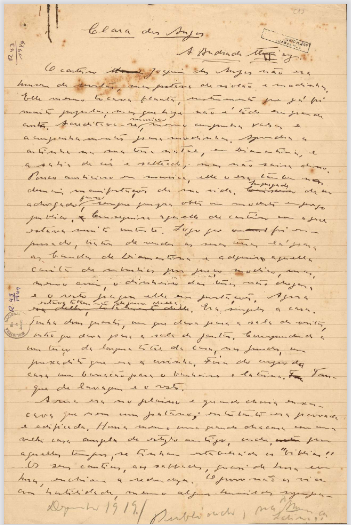
\includegraphics[width=5cm]{./images/PNLD0001-09.png}\\
\textit{Foto do autor}}

Importante ressaltar a maneira como o escritor reagiu aos jornais
argentinos. Interpretou aquilo que seria ofensivo de maneira a valorizar
nosso parentesco com os macacos. O que teria levado o autor a agir dessa
forma e não de outra? Não seria mais natural, principalmente vindo de um
escritor como Lima Barreto, uma crônica revoltada? Não estaria sendo
irônico?

Outro ponto importante a ser desenvolvido junto aos alunos e alunas,
diz respeito a maneira como Lima Barreto se posicionava diante do
Futebol. Na seção dedicada às crônicas, selecionamos uma série de textos
que Lima Barreto escreveu contra o futebol e que podem servir de
subsídios para um maior aprofundamento da atividade.

\paragraph{\textit{Pós"-leitura}}

O racismo e o preconceito de cor, tal como se configuram no Brasil,
têm uma relação direta e fundante na experiência da escravidão, que
formalmente foi abolida em nosso país a partir de 13 de maio de 1888.
Importante que os alunos e alunas terminem essa proposta de atividade em
condições de relacionarem todos esses aspectos que foram aparecendo ao
longo das pesquisas e da leitura do texto com a herança escravista de
nosso país. Que sejam capazes de responder a questões como: o que foi a
escravidão? Qual a relação entre escravidão, raça, racismo e preconceito
de cor? Como essas estruturas formativas de nossa nação ainda operam no
cotidiano a partir de diferentes perspectivas: no encarceramento, no
assassinato de jovens negros e moradores das periferias, nos postos mais
baixos de trabalho, etc.

Uma atividade específica em relação à crônica pode ser solicitada aos
alunos e alunas a partir da prática, muito difundida de em várias
equipes de futebol, de passar ``pó de arroz'' no rosto dos jogadores
``de cor''. Quais equipes mantinham essa prática? A partir de quando o
futebol profissional deixou de segregar racialmente os jogadores, quais
as equipes que iniciaram esse movimento?

%\begin{enumerate}
%\def\labelenumi{\arabic{enumi})}
%\item
  %Para o conto {\textit{O pecado}}
%\end{enumerate}

\subsubsection{\textit{O pecado}}

\paragraph{\textit{Pré"-leitura}}

Como atividade de pré"-leitura indicamos para que os alunos e alunas
assistam ao vídeo ``Lima Barreto'', da série \emph{Heróis de Todo
Mundo}\footnote{Link para acesso ao vídeo:
  \url{https://www.youtube.com/watch?v=e2mZHmSo_c4}}. Como complemento
ao vídeo, professores e professoras podem fazer uma discussão sobre a
importância de Lima Barreto e de sua literatura para o combate ao
racismo e ao preconceito de cor no Brasil.

\paragraph{\textit{Leitura}}

Ao longo da atividade de leitura podem ser retomadas os recursos
técnicos que normalmente aparecem em um conto 1) O tipo de narrador (em
terceira pessoa); 2) Personagens (São Pedro, o Supremo, o Guarda"-livros,
Anjos mensageiros, P. L. C.); 3) O conflito que alicerça a narrativa (a
decisão de se mandar ou não alguma alma ao purgatório); 4) As dimensões
de tempo/espaço (o Céu, apresentado como uma repartição burocrática; 5)
Clímax (desenlace da história).

O conto apresenta uma atmosfera um tanto religiosa. O autor manipula um
pouco do imaginário que fomos criando das ideias de Deus (o Supremo), de
São Pedro, que recebe as almas no céu, bem como das instâncias as quais
as almas teriam como paradeiro, após a morte. Aqui pode ser discutida a
ideia de ``justiça divina'', tal qual aparece na religião Cristã. O que
significa para a religião cristã o purgatório? Outra ideia importante
que pode estimular a discussão seria a apresentação de outras
manifestações religiosas e como elas encaram a ideia da morte.

\begin{figure}[ht!]
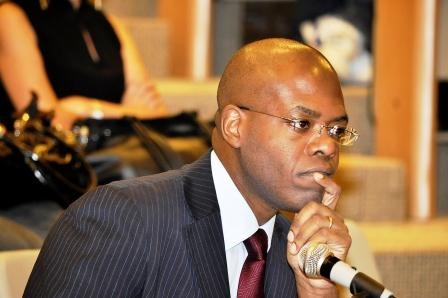
\includegraphics[width=\textwidth]{./images/PNLD0001-13.png}
\end{figure}

Esse conto também proporciona uma ótima alegoria para se inserir o tema
do racismo estrutural. Um ponto de partida importante para que os
professores e professoras realizem essa leitura seria através do livro
``O que é racismo estrutural'' de autoria de Silvio Almeida.

\paragraph{\textit{Pós"-leitura}}

Como atividade de pós"-leitura, sugerimos um trabalho pautado na
necessidade de se combater a discriminação racial. Um bom caminho seria
os alunos e alunas pesquisarem sobre movimentos de luta contra a
situação de subjugação da população afro"-brasileira, por exemplo: os
Quilombos, o Movimento Abolicionista, o Movimento Negro Unificado.
Outras pesquisas podem ser desenvolvidas no âmbito das conquistas legais
e jurídicas, tais como: a \textit{Lei nº 7.716} de 5 de janeiro de 1989
(conhecida como ``Lei Caó''); a \textit{Lei 9.029} de 13 de abril de
1995; o \textit{Estatuto da Igualdade Racial} (Lei nº 12288, de 20 de
julho de 2010), que estabelece as cotas raciais em diversas esferas da
atividade social e a \textit{Lei 10.639} de 9 de janeiro de 2003, que
instituiu a obrigatoriedade na educação básica do ``estudo da história
da África e dos africanos, a luta dos negros no Brasil, a cultura negra
brasileira e o negro na formação da sociedade nacional, resgatando a
contribuição do povo negro nas áreas social, econômica e política
pertinentes à história do Brasil''.

Outra atividade importante seria estimular cada vez mais os alunos e
alunas a conhecerem outros escritores e escritoras afro"-brasileiros,
tais como Luiz Gama, Machado de Assis, Maria Firmina dos Reis, Carolina
de Jesus, Conceição Evaristo, entre tantos outros e outras.

\marginnote{\footnotesize\textbf{EM13LGG703}\\
Utilizar diferentes linguagens, mídias e ferramentas digitais em processos de produção coletiva, colaborativa e projetos autorais em ambientes digitais.\\\medskip
\textbf{EM13LGG704}\\
Apropriar-se criticamente de processos de pesquisa e busca de informação, por meio de ferramentas e dos novos formatos de produção e distribuição do conhecimento na cultura de rede.\\\medskip
\textbf{EM13LP16}\\
Utilizar softwares de edição de textos, fotos, vídeos e áudio, além de ferramentas e ambientes colaborativos para criar textos e produções multissemióticas com finalidades diversas, explorando os recursos e efeitos disponíveis e apropriando-se de práticas colaborativas de escrita, de construção coletiva do conhecimento e de desenvolvimento de projetos. Competências específicas: 7\\\medskip
\textbf{EM13LP36}\\
Conhecer e analisar diferentes projetos editorias – institucionais, privados, públicos, financiados, independentes etc. –, de forma a ampliar o repertório de escolhas possíveis de fontes de informação e opinião, reconhecendo o papel da mídia plural para a consolidação da democracia. Competências específicas: 2\\\medskip
\textbf{EM13LP44}\\
Analisar, discutir, produzir e socializar, tendo em vista temas e acontecimentos de interesse local ou global, notícias, fotodenúncias, fotorreportagens, reportagens multimidiáticas, documentários, infográficos, podcasts noticiosos, artigos de opinião, críticas da mídia, vlogs de opinião, textos de apresentação e apreciação de produções culturais (resenhas, ensaios etc.) e outros gêneros próprios das formas de expressão das culturas juvenis (vlogs e podcasts culturais, gameplay etc.), em várias mídias, vivenciando de forma significativa o papel de repórter, analista, crítico, editorialista ou articulista, leitor, vlogueiro e booktuber, entre outros. Competências específicas: 1, 3 }

\subsection{Denunciando a Violência contra as mulheres}


\paragraph{Conteúdo} Na \emph{Antologia de crônicas e contos de Lima
Barreto} inserimos uma seção intitulada ``Violência contra as mulheres''
em que selecionamos algumas crônicas e artigos jornalísticos nos quais o
autor denunciou aquilo que conhecemos hoje em dia como ``feminicídio''.
Para esta atividade pretende"-se trabalhar junto às alunas e alunos essa
questão bastante complexa e persistente na sociedade brasileira. Os
textos podem ser trabalhados em conjunto ou individualmente.

\paragraph{Objetivos} Objetiva"-se com essa atividade despertar um olhar
crítico dos alunos em relação à desigualdade de gênero e à violência
contra as mulheres, cuja dimensão extrema é a prática do crime de
feminicídio. Mostrar que Lima Barreto, com sua prosa militante,
frequentemente escrevia contra as práticas de discriminação e violência,
tanto através das crônicas e artigos de jornal, quanto em sua prosa de
ficção.

\paragraph{Justificativa} Apesar de todos os avanços e conquistas nas
áreas jurídicas, econômicas, políticas e socias, fruto das lutas
empreendidas pelas mulheres, ainda observamos uma sociedade extremamente
desigual e marcada pela violência e opressão contra as mulheres. Sem
contar a situação opressiva em relação à outras e outros segmentos da
população, como as pessoas \textsc{lgbtqia}+, as etnias constituídas pelos povos
originários, os quilombolas.

\paragraph{Metodologia} Usaremos como modelo a crônica {\textit{Lavar
a honra, matando?}}, entre os vários textos através dos quais o escritor
denunciou a violência contra as mulheres. Para essa atividade também
propomos um diálogo com as áreas de História, Sociologia e Antropologia,
dialogo que pode trazer grandes contribuições para o entendimento mais
amplo do tema: 1) As relações entre homens e mulheres numa dimensão
Antropológica, sob a ótica do parentesco, da família patriarcal, da
divisão dos gêneros já a partir da infância (meninos usam azul, meninas
usam rosa; 2) Dimensões das desigualdades de gênero, sob uma perspectiva
Sociológica --- as mulheres ganham menos que os homens, ocupam lugares
inferiores nas hierarquias da maioria das instituições e empresas,
exercem a dupla ou tripla jornada; 3) Numa perspectiva Histórica, o
processo de lutas pela igualdade de direitos e pela emancipação das
mulheres. Vejamos alguns pontos que podem ser desenvolvidos a partir da
crônica selecionada:

\subsection{\textit{Pré"-leitura}}

Com o advento da internet e das redes sociais, os casos de violência
contra as mulheres ganharam uma ampla divulgação. Em 2015, foi aprovada
a Lei~13.104/15, conhecida como ``Lei do feminicídio'', que endurece a
pena contra os assassinos de mulheres. Mas esses fatos não vêm impedindo
que as estatísticas desse tipo de crime aumentem. Como atividade de
pré"-leitura, sugerimos que os professores e professoras estimulem os
alunos e alunas a pesquisarem o tema, a partir de casos mais recentes.
Importante, também, que haja uma explanação sobre os tipos de violência
que as mulheres sofrem, as motivações, os agressores. Como sugestão,
indicamos o vídeo ``Violência contra a mulher: dados e
definições.''\footnote{O vídeo pode ser acessado a partir do link:
  \url{https://www.youtube.com/watch?v=SLfF9aAntQU}}

\begin{figure}[ht!]
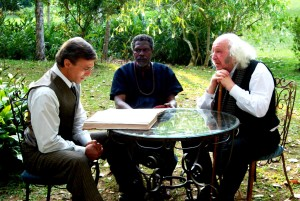
\includegraphics[width=\textwidth]{./images/PNLD0001-10.png}
\end{figure}

\subsection{\textit{Leitura}}
	
A crônica {\textit{Lavar a honra, matando?}} é um dos vários textos
que Lima Barreto escreveu sobre o tema. Ela é importante porque mostra a
situação extremamente desfavorável das mulheres em relação a seus
agressores, que tinham amparo legal para os proteger. Nosso antigo
Código Penal, que vigorou de 1890 até 1940, versava, em seu artigo 27,
que poderia ser excluída a ilicitude dos atos cometidos por pessoas que
``\emph{se acharem em estado de completa privação de sentidos e de
inteligência no ato de cometer o crime}''. Era quase como um ``direto de
matar'', uma vez que fosse provada a alteração do estado emocional do
criminoso. Esse mesmo artigo era utilizado por muitos advogados e
juristas para justificar a chamada ``\emph{legítima defesa da honra}'',
quando algum marido descobria situações de adultério por parte da
esposa. Mas, o mesmo critério não valia para as mulheres. Os homens
adúlteros não se enquadravam na legislação. Este é o pano de fundo e o
contexto histórico e jurídico que Lima Barreto está descrevendo. Embora
o texto não diga com clareza, é muito provável que a absolvição do
assassino, que o próprio Lima Barreto endossou, tenha sido em função da
``legitima defesa da honra''. O autor não diz que absolveu o réu em
função da tal ``Lei'', mas sim por ter se comovido com a mãe do
assassino, o que é algo bastante controverso e causou arrependimento.
Lima Barreto usa a palavra ``uxoricida'' para descrever os assassinos de
mulheres, que era um termo jurídico utilizado na época. É importante
falar sobre o significado dessa palavra e a partir dela, professores e
professoras podem desenvolver atividades sobre as mudanças das leis de
proteção à mulher no país. Por exemplo, as leis que tipificam o estupro
ou a importunação sexual, que tiveram mudanças nos últimos anos.

Outro ponto importante que a crônica apresenta, pode ser explorado a
partir de um caso recente, que ganhou grande repercussão através da
internet. Conhecido como ``Caso Mariana Ferrer'', trouxe a questão da
``culpabilidade da vítima'', um sentimento que ainda persiste em nossa
sociedade, quando a vítima da agressão é supostamente acusada de ter
provocado o ato de violência. Esse caso é importante, pois mostra um
juiz e um advogado tentando absolver o réu a partir da ideia de que a
vítima teria sido responsável por ter sido violentada. Falou"-se na época
da tentativa de se criar uma nova tipificação legal para os casos de
estupro --- o ``estupro culposo''.

Outro ponto importante a ser discutido a partir da leitura dessa crônica
diz respeito ao caráter estrutural e longevo da prática de violência
contra as mulheres. A leitura dos outros textos presentes na seção
``Violência contra as mulheres'' pode ser um bom caminho para despertar
a percepção dos estudantes sobre o caráter histórico e cultural do
problema. Caso os professores e professoras desejem aprofundar ainda
mais essa questão, sugerimos a leitura do livro ``Entre a agulha e a
caneta: a mulher na obra de Lima Barreto'', da pesquisadora Eliane
Vasconcellos.

\subsection{\textit{Pós"-leitura}}

Espera"-se que a partir dessa atividade os alunos e alunas criem uma
sensibilidade mínima para enxergar que a violência contra a mulher é um
problema extremamente grave de saúde pública e responsável pelo
adoecimento, internação e morte de muitas mulheres. Saber, entre outras
coisas, que o Brasil é o quinto país com maior taxa de feminicídio no
mundo, possuindo índices epidêmicos de violência contra a mulher, sendo
que, grande parte dessas mulheres, são assassinadas por parceiros ou
ex"-parceiros. Mesmo que a mulher saia desse contexto de violência, os
prejuízos emocionais e psicológicos podem acompanhá-la por muito tempo,
sendo necessário a busca de ajuda profissional.

Outro caso a ser explorado e requisitado como pesquisa para os alunos e
alunas é a história de Maria da Penha, que lutou por anos para que seu
agressor/marido fosse punido. Precisou recorrer a instancias
internacionais para chamar a atenção para seu caso. Alguns materiais que
podem servir de apoio, para atividades ou trabalhos, em grupo ou
individuais: O livro escrito pela própria Maria da Penha, lançado em
1994, ``Sobrevivi...posso contar'', além dos materiais disponíveis no
site do Instituto Maria da Penha\footnote{Link para acesso:
  \url{https://www.institutomariadapenha.org.br/quem"-e"-maria"-da"-penha.html}}
ou do Instituto da Mulher Negra -- Geledés\footnote{Link para acesso:
  \url{https://www.geledes.org.br}}

\section{Para aprofundar}

Afonso Henriques de Lima Barreto, seguramente um dos maiores escritores
de nossa literatura, nasceu na cidade do Rio de Janeiro, no dia 13 de
maio de 1881. Era filho de Amália Augusta Pereira de Carvalho,
professora de escola primária, e do tipógrafo João Henriques de Lima
Barreto.

O futuro escritor recebeu, pelo enorme esforço de sua mãe e de seu pai,
uma educação de excelente qualidade. Estudou em ótimas escolas e mesmo
com o falecimento de sua mãe, quando ele tinha apenas seis anos de
idade, continuou no trilho dos estudos.

Começou sua carreira literária quando era estudante de Engenharia Civil,
na Escola Politécnica, escrevendo pequenos textos humorísticos e
satíricos, alguns dos quais tinham como personagens os próprios
professores da instituição.

\marginnote{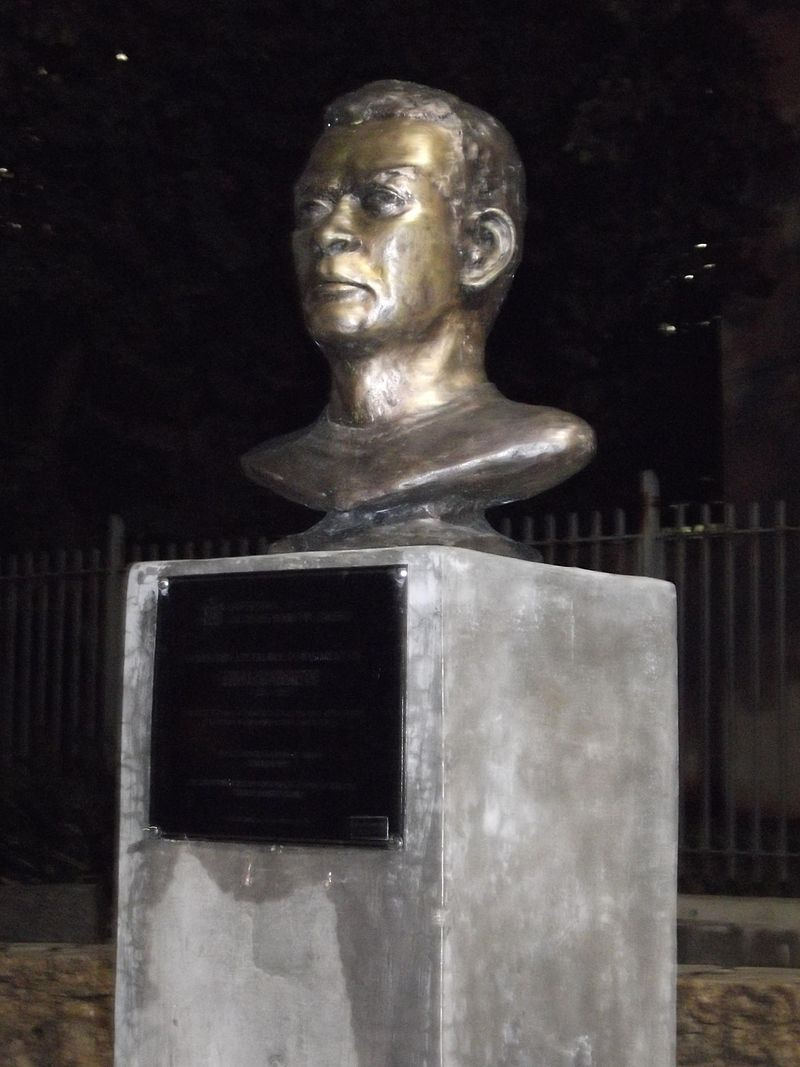
\includegraphics[width=5cm]{./images/PNLD0001-11.png}\\
\textit{Foto do autor}}

Por conta de uma grave doença psiquiátrica sofrida por seu pai, que o
deixou impossibilitado de trabalhar, e de sucessivas reprovações na
faculdade, Lima Barreto foi obrigado a abandonar o curso de Engenharia.
Prestou concurso público e começou a trabalhar como amanuense na
Secretária do Arsenal de Guerra, uma repartição burocrática do Exército.

Seu primeiro livro, \emph{Recordações do escrivão Isaías Caminha}, foi
publicado em 1909. A partir daí, Lima Barreto começou a despertar o
incômodo de muitos setores da intelectualidade. Seu livro de estreia
apresenta uma forte denúncia contra o preconceito de cor, além de tecer
severas críticas ao jornalismo, à imprensa e à política da ``Primeira
República''.

De origem afrodescendente --- suas avós materna e paterna foram mulheres
escravizadas"-libertas --- experimentou na pele a discriminação racial e
os limites impostos pelo racismo para quem desejava, como ele, uma
carreira bem sucedida, primeiro como Engenheiro, depois como escritor e
jornalista. Sua literatura, bem como sua atividade jornalística, trazem
as marcas do inconformismo social, a revolta contra os preconceitos e
injustiças, principalmente contra o racismo, que combateu abertamente,
seja através de artigos para a imprensa ou de sua prosa de ficção.

Foi um dos primeiros escritores a perceber, junto a Euclides da Cunha,
autor de \emph{Os Sertões}, e de Graça Aranha, com o romance
\emph{Canaã}, ambos publicados em 1902, que o advento da Abolição (1888)
e a Proclamação da República (1889) não trouxeram nenhum tipo de alívio
para a população pobre, sobretudo para os descendentes de escravos.
Combateu a ``República'', que considerava um arranjo de poderosos e
politiqueiros de interesses mesquinhos, bem como tudo aquilo que ajudava
a sustentar ideologicamente um empreendimento que na prática não tinha
nada de democrático ou republicano. Muitos historiadores dizem ser
impossível compreender a essência da chamada ``Primeira República''
(1889--1930) sem estudar a obra de Lima Barreto.

Mas não foi somente no campo das ideias políticas e sociais que o autor
se destacou. Sua obra foi escrita num momento de efervescência cultural
e modernização do país, principalmente de algumas capitais como Rio de
Janeiro, São Paulo, Belo Horizonte, Manaus, Belém, entre outras. Era o
tempo da \emph{belle époque}, cuja literatura representativa foi
definida por Antonio Candido nos seguintes termos:

\begin{quote}
... era sobretudo uma conservação de formas cada vez mais vazias de
conteúdo; uma tendência a repisar soluções plásticas que, na sua
superficialidade, conquistaram por tal forma o gosto médio, que até hoje
representam para ele a boa norma literária. Uma literatura para a qual o
mundo exterior existia no sentido mais banal da palavra, e que por isso
mesmo se instalou num certo oficialismo graças, em parte, à ação
estabilizadora da Academia Brasileira. As letras, o público burguês e o
mundo oficial se entrosavam numa harmoniosa mediania.\footnote{\textsc{candido},
  Antonio. ``Literatura e cultura de 1900 a 1945''. In: \emph{Literatura
  e Sociedade}. Rio de Janeiro: Ouro sobre Azul, 2006, p. 125.}
\end{quote}

A literatura de Lima Barreto, no entanto, foi exatamente o oposto da
``literatura oficial'' praticada na \emph{belle époque} carioca. Ao
desobedecer às regras do bem escrever e do ``bom gosto literário'',
colocou a prosa de ficção brasileira em um outro patamar estético. Ele
mesmo definiu sua escrita como ``literatura militante'', um meio de
atuação política e estética.

Muitos estudiosos da literatura se renderam ao conceito de
``Pré"-modernismo'' para tentar dar conta das transformações estéticas
ocorridas naquele período, compreendido mais ou menos entre o último
quarto do século \textsc{xix} e as duas primeiras décadas do século \textsc{xx}. Trata"-se
de um momento em que as escolas literárias já não tinham tanto fôlego
quanto antes --- Romantismo, Parnasianismo, Simbolismo, Naturalismo --- e
cediam lugar a formas cada vez mais híbridas e inovadoras de composição.
As chamadas vanguardas artísticas e o surgimento de novas tecnologias,
como as revistas ilustradas, o jornalismo empresarial, o telégrafo, a
expansão da eletricidade, o rádio, o cinema, enfim, o próprio momento de
modernização do país (industrialização, urbanização, rápidas mudanças
nos costumes), todo esse arcabouço de novidades e invenções operou e
exigiu uma nova mentalidade estética, uma maneira outra de percepção da
realidade e dos costumes.

Muitos escritores, que na época da \emph{belle époque} fizeram um enorme
sucesso --- Coelho Neto, Figueiredo Pimentel, Afrânio Peixoto, Medeiros e
Albuquerque, para citarmos apenas alguns --- quase não são lembrados ou
conhecidos hoje em dia. Lima Barreto teve seu nome quase esquecido após
sua morte, ocorrida no dia 01 de novembro de 1922. Sua obra caiu num
limbo de quase três décadas e só voltou a ser reeditada graças aos
esforços de Francisco de Assis Barbosa que, além de escrever a grande
biografia do autor, \emph{A vida de Lima Barreto}, em 1952, também
coordenou a edição das \emph{Obras completas de Lima Barreto,} em 17
volumes, publicados em 1956 pela editora Brasiliense. Somente a partir
daí o nome e a obra do grande escritor carioca voltou a fazer parte do
patrimônio das letras brasileiras.

A crítica literária oscilou bastante até reconhecer em Lima Barreto um
escritor de primeiro escalão. Desde seus primeiros romances,
\emph{Recordações do escrivão Isaías Caminha} (1909), \emph{Triste fim
de Policarpo Quaresma} --- publicado primeiramente em folhetins, no
Jornal do Comércio, em 1911 e depois editado em livro em 1915 --- e
\emph{Numa e a Ninfa} (1915), o escritor foi apreciado ora como um
grande prosador e crítico da sociedade, ora como um artista ``menos
realizado''. Muitos estudiosos consideraram que Lima Barreto exagerou um
pouco no ``autobiografismo'', principalmente em seu romance de estreia,
como também no excesso de coloquialismos, num certo ``desleixo''
artístico, na irregularidade do estilo, que oscila entre uma linguagem
jornalística, sociológica, anárquica. Tudo isso foi encarado como
``incorreções da forma'', que sempre teve como exemplares os romances e
contos de Machado de Assis.

\begin{figure}[ht!]
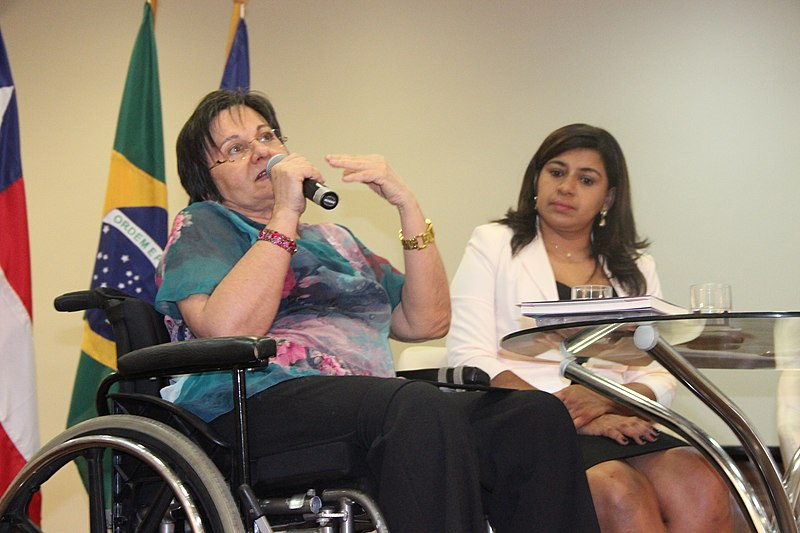
\includegraphics[width=\textwidth]{./images/PNLD0001-15.png}
\end{figure}

Lima Barreto foi um escritor de outra geração, uma após a do autor de
\emph{Memórias póstumas de Brás Cubas} (1881), ou seja, foi um escritor
do período republicano e pós"-abolicionista. Nesse sentido, tanto do
ponto de vista formal, quanto temático, Lima Barreto assumiu uma posição
renovadora, confrontadora, pois a literatura não podia mais ser um
privilégio das elites letradas, nem se abster dos problemas sociais
concretos pelos quais a população em sua grande maioria passava,
sobretudo os descendentes de escravos.

A própria sociedade havia mudado muito rapidamente ao longo dos vinte
primeiros anos do século \textsc{xx}. As antigas elites do Império, compostas por
fazendeiros escravagistas, foram substituídas por uma nova elite cada
vez mais citadina, moderna e financista. Mesmo os chamados barões do
café compunham uma nova camada social, mais ligada ao desenvolvimento de
setores modernos, como ferrovias, portos, eletricidade, urbanismo,
arquitetura (palacetes, teatros, cinemas). No campo político, as
promessas de uma nova era, com a Proclamação da República, ficaram muito
aquém da realidade. O que se via era um conchavo de oligarquias se
alternando no poder, um acúmulo cada vez maior de riquezas, enquanto o
grosso da população vivia em condições semelhantes, senão piores, que na
época do Império.

Lima Barreto não só viveu tudo isso, mas compôs um retrato crítico e
fiel da época, sem deixar de se posicionar ao lado dos desfavorecidos.
Por isso, nunca participou como membro efetivo da ``elite literária'' da
época. Com fama de ``boêmio'' e ``beberrão'', passou por períodos de
internação em Hospitais psiquiátricos, dos quais temos algumas das mais
dilacerantes páginas testemunhais, conforme aparecem em \emph{O
cemitério dos vivos}, romance que deixou inacabado, e no \emph{Diário do
Hospício}, escrito nas épocas de internação.

Como salientamos um pouco acima, suas obras --- crônicas, contos,
novelas, romances, diários e memórias --- não são apenas relatos
instantâneos de uma realidade que se apresentava hostil ao escritor. Com
o tempo, a pecha de escritor ``desleixado'' foi ficando superada. Hoje
em dia, não há dúvidas em relação a um livro como \emph{Triste fim de
Policarpo Quaresma} figurar como um dos maiores de nossa literatura. E
mesmo livros que não foram bem recebidos na época de publicação,
\emph{Recordações do escrivão Isaías Caminha} ou \emph{Vida e Morte de
M. J. Gonzaga de Sá} (1919) cada vez mais são objeto de estudos e novas
interpretações. Não ficaram estagnados no tempo, como ficou a grande
maioria dos ``famosos'' e mais lidos escritores seus contemporâneos.

Lima Barreto escreveu numa época em que a literatura tinha um parentesco
fortíssimo com os jornais. Normalmente, antes de ganhar uma edição em
livro, os textos apareciam primeiramente nas edições dos jornais e
revistas. A atividade jornalística não havia se desenvolvido como hoje
em dia e boa parte do que era escrito nos jornais vinha das mãos dos
escritores literatos. A profissão de \emph{jornalista}, como nós a
conhecemos atualmente, estava dando os primeiros passos.

Conforme salientou o sociólogo Sérgio Miceli, em seu livro \emph{Poder,
Sexo e Letras na República Velha}: ``toda a vida intelectual era
dominada pela grande imprensa, que constituía a principal instância de
produção cultural da época e que fornecia a maioria das gratificações e
posições intelectuais.''\footnote{Sérgio Miceli. \emph{Poder, Sexo e
  Letras na República Velha}. São Paulo: Perspectiva, 1977, p.\,15.}

A principal atividade dos escritores era o jornalismo, onde conseguiam
uma renda extra ``cada vez mais indispensável'', além de, alcançarem
``salários melhores, sinecuras burocráticas e favores
diversos.''\footnote{Idem, p. 77.} Não faltavam nos principais jornais e
revistas da época seções destinadas à literatura, além do espaço cada
vez maior aberto aos escritores em diversas colunas dos jornais, ou até
mesmo cargos de redatores e diretores.

\begin{figure}[ht!]
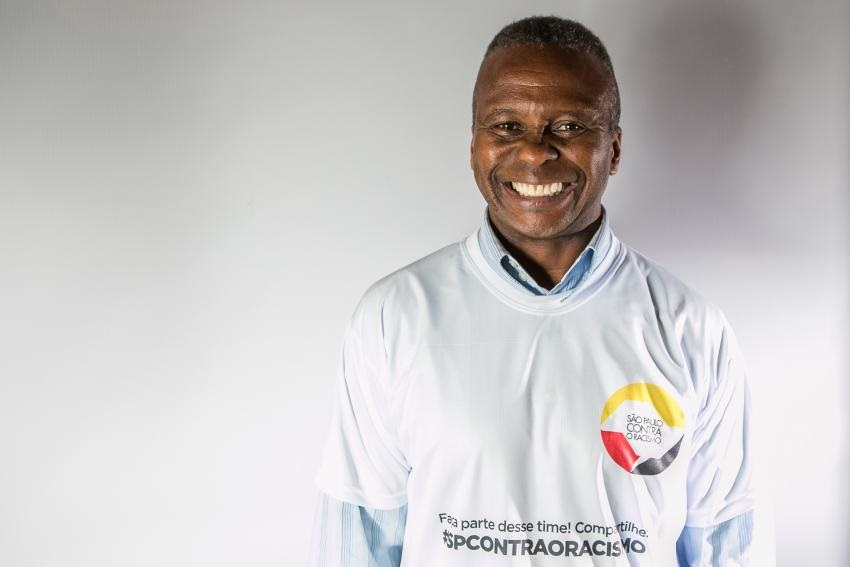
\includegraphics[width=\textwidth]{./images/PNLD0001-12.png}
\end{figure}

Jornais e revistas ilustradas foram os grandes veículos para os textos
de ficção, em suas mais diversas vertentes. Conforme observou Nelson
Werneck Sodré: ``os homens de letras buscarem no jornal o que não
encontravam no livro: notoriedade, em primeiro lugar; um pouco de
dinheiro, se possível.''\footnote{Nelson Werneck Sodré. \emph{A História
  da Imprensa no Brasil}. Rio de Janeiro: Civilização Brasileira, 1966,
  p. 297.}

Este processo aconteceu primeiro como estratégia por parte de alguns
donos de jornais para conseguirem mais leitores e assinantes, além de
diversificar o material jornalístico, sempre voltado para assuntos
políticos e administrativos.

Na metade do século \textsc{xix} a literatura já tinha ocupado um lugar de
destaque na imprensa brasileira. O gênero ``folhetim'' fazia parte dos
principais jornais da época. Junto ao folhetim, a crônica também foi se
desenvolvendo. Como demonstra Marcus Vinicius Soares, a crônica é
anterior ao folhetim e ``já fazia parte do universo jornalístico, sempre
acompanhada pelo epíteto designativo de sua matéria específica: crônica
dramática, crônica musical, crônica literária, etc.''\footnote{Marcus
  Vinicius Soares. \emph{João do Rio e a nova esfera da crônica no
  século \textsc{xx}}. São Paulo: Intermeios, 2016, p. 122.}

Já no século \textsc{xx}, o jornalismo passa a ser uma empresa especializada, com
diferenciação nas modalidades de texto. Na diagramação dos jornais,
criam"-se espaços dedicados à literatura. Surgem os 'suplementos
literários', como sintoma desta nova relação estabelecida entre
jornalismo e literatura.

De estreitas relações com o jornalismo foi também o desenvolvimento do
gênero conto, em sua modalidade moderna, ou seja, escrita e voltada para
um público leitor. Nesse ambiente literário, no entanto, o conto também
era considerado algo esteticamente secundário, um ``treinamento'' para
narrativas de maior fôlego. Embora já tivéssemos desenvolvida no Brasil
uma tradição de contadores de histórias oriundos da cultura oral, o
conto literário ainda era visto como uma literatura de menor valor
artístico.

Tradicionalmente já tínhamos o hábito do ``causo'' e da ``anedota''; dos
indígenas conhecemos suas lendas, mitos e cosmologias; as escravas e
amas"-de"-leite povoaram o imaginário dos brancos com suas histórias
cheias de seres fantásticos, magias, feiticeiros, entidades do panteão
religioso, etc. Conforme demonstra a pesquisadora Sônia Brayner: ``a
oralidade do contar foi criando e embalando os embriões de personagens e
tramas mais tarde corporificados e desenvolvidos pela literatura
escrita''\footnote{Sônia Brayner. ``O conto de Machado de Assis''. In:
  \emph{O conto de Machado de Assis -- Antologia}. Rio de Janeiro:
  Civilização Brasileira, 1981, p. 06.}.

Foi neste contexto que Lima Barreto desenvolveu sua produção literária.
Incorporou em sua produção as novas técnicas expressivas, que surgiram
das relações entre literatura e jornalismo. E também nossa tradição
oral, que junto à dicção jornalística de sua prosa, consolidou uma forma
de escrita bastante moderna para a época. Percebemos muito bem esses
traços em narrativas como {\textit{O gambá}}, {\textit{A
Pescaria}}, {\textit{Rocha, o guerreiro}}, {\textit{O homem
que sabia javanês}}, que escolhemos para compor a \emph{Antologia},
entre outras tantas criações.

Além de cronista e contista, Lima Barreto foi um grande romancista e
considerado por muitos pesquisadores como um dos protótipos do
escritor"-jornalista. A atualidade de sua obra é algo a ser levado em
consideração, principalmente pelos temas que abordou,
impressionantemente presentes e atuantes nos dias de hoje, e pela forma
renovadora de sua literatura, que só muitas décadas depois de sua morte
teve o seu devido reconhecimento.

\section{Sugestões de referências complementares}

\textbf{Lima Barreto -- \emph{De Lá Pra Cá} }\\
Link: \url{https://www.youtube.com/watch?v=M4roOVqpotY}

A série ``de Lá Pra Cá'', produzida pela \textsc{tv} Escola, tem como objetivo
apresentar as principais figuras da literatura brasileira. Este programa
foi dedicado à vida e obra de Afonso Henriques de Lima Barreto. Com uma
linguagem de fácil compreensão e ótimas entrevistas, o vídeo se
constitui como uma boa ferramenta didática para uma introdução ao autor.

\noindent\textbf{Lima Barreto \emph{-- Um grito brasileiro}. }\\
Link: \url{https://www.youtube.com/watch?v=Bas_Os1pv1o\&t=1190s}

Programa Mestres da Literatura, \textsc{tv} Escola. Dir. Mônica Simões. O vídeo
apresenta um amplo panorama da vida, obra e época de Lima Barreto. Com
leituras de trechos de seus livros e depoimentos de especialistas em sua
obra.

\begin{figure}[ht!]
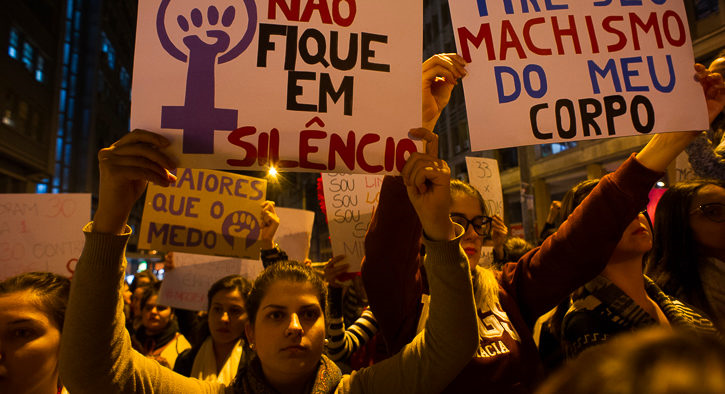
\includegraphics[width=\textwidth]{./images/PNLD0001-14.png}
%\caption{Silvio Almeida}
\end{figure}

\section{Bibliografia comentada}

%\begin{enumerate}
%\def\labelenumi{\arabic{enumi})}
%\item
  %\textit{Sobre Lima Barreto}
%\end{enumerate}

\subsection{Sobre Lima Barreto}

\textsc{barbosa}, Francisco de Assis. \emph{A vida de Lima Barreto: 1881-1922}.
11 ed. Belo Horizonte: Autêntica Editora, 2017. Principal biografia
sobre a vida de Lima Barreto. Publicado em 1952, essa obra se constitui
como o ponto de partida para a redescoberta de Lima Barreto. Assis
Barbosa também foi o organizador das \emph{Obras completas de Lima
Barreto,} publicadas em 1956, em 17 volumes, pela editora Brasiliense. O
livro \emph{A vida de Lima Barreto}, foi escrito de modo a
interrelacionar eventos da vida pessoal do autor com diversas passagens
de sua obra ficcional, assim como a contextualização da época, na
verdade um grande painel histórico, rico em detalhes e informações que
compõem um quadro muito completo desse grande escritor brasileiro.

\textsc{prado}, Antonio Arnoni. \emph{Lima Barreto: uma autobiografia literária}.
São Paulo: Editora 34, 2012. Um dos maiores estudiosos da obra de Lima
Barreto, o crítico Antonio Arnoni apresenta nesse livro magistral,
através de trechos retirados de toda a obra do escritor carioca, o
percurso formativo da sensibilidade artística e literária do autor. Com
um misto de prosa autobiográfica, fontes de crítica e doutrina
literária, pontos de vista assumidos em relação à arte e a literatura,
costuradas com muito engenho pelo ensaísta, essa obra abre as portas
para compreendermos as escolhas de Lima Barreto, a maneira pela qual foi
compondo sua visão de mundo, bem como o modo de expressá"-la, através de
sua prosa afiada e revolucionária.

%\begin{enumerate}
%\def\labelenumi{\arabic{enumi})}
%\item
  %\textit{A obra de Lima Barreto e o estudo da sociedade brasileira}
%\end{enumerate}

\subsection{A obra de Lima Barreto e o estudo da sociedade brasileira}

\textsc{sevcenko}, Nicolau. \emph{Literatura como missão: tensões sociais e
criação cultural na Primeira República}. São Paulo: Brasiliense, 1999.
Estudo amplo e profundo sobre a Primeira República. As transformações
sociais, econômicas e culturais são abordadas com uma crítica severa,
num diálogo profícuo com a obra de Euclides da Cunha e Lima Barreto.

\textsc{resende}, Beatriz. \emph{Lima Barreto e o Rio de Janeiro em Fragmentos}.
São Paulo: Editora Autêntica, 2016. O apresenta um grande painel da
cidade do Rio de Janeiro, sob a ótica do cronista Lima Barreto. A partir
dessa leitura, os textos do escritor carioca ganham mais vida e um
sentido de reciprocidade entre autor e cidade, entre o escritor
marginalizado e a metrópole em amplo e acelerado processo de
modernização, cada vez mais excludente e segregadora.

\textsc{cury}, M. Zilda Ferreira.~\emph{Um mulato no reino de
Jambom}\textit{~}(As classes sociais na obra de Lima Barreto). São
Paulo: Cortez, 1981. Trata"-se de um dos primeiros e mais fecundos livros
escritos sobre a obra de Lima Barreto e as relações entre sua literatura
e a sociedade de seu tempo. O ponto central da análise da autora é o
lugar social ocupado por Lima Barreto na estrutura de classes da
sociedade brasileira do início do século \textsc{xx}. Esse lugar, que hoje
denominamos de ``classe média'', permitiu ao autor, principalmente por
ser negro, denunciar todos os tipos de violência a que estavam
submetidas as classes populares, ao mesmo tempo em que estimulava o
escritor a ascender na hierarquia social.

\textsc{figueiredo}, Carmem Lucia Negreiros de. \emph{Lima Barreto e o fim do
sonho republicano}. Rio de Janeiro: Editora Tempo Brasileiro, 1995. Uma
das maiores estudiosas sobre a obra de Lima Barreto, Carmem Negreiros
apresenta neste estudo a maneira pela qual o autor desmistifica, através
da ironia, as principais ideologias da época, que apresentavam uma
cidade moderna e nos trilhos do progresso. Trata"-se do primeiro dentre
os vários trabalhos de Carmem Negreiros dedicados a Lima Barreto, dentre
os quais ainda destacamos: \emph{Trincheiras de sonho: Ficção e cultura
em Lima Barreto}. Rio de Janeiro: Editora Tempo Brasileiro, 1998.

%\begin{enumerate}
%\def\labelenumi{\arabic{enumi})}
%\item
  %\begin{quote}
  %\textit{Sobre o período histórico de Lima Barreto}
  %\end{quote}
%\end{enumerate}

\subsection{Sobre o período histórico de Lima Barreto}

\textsc{carvalho}, José Murilo de. \emph{Os bestializados: o Rio de Janeiro e a
República que não foi}. São Paulo: Companhia das Letras, 1987. Um dos
mais completos estudos sobre o nosso primeiro período republicano, o
livro traz uma abordagem história, social, literária, cultural e
política. O autor perpassa por esses campos para reconstruir todo um
imaginário cotidiano, político e social da chamada Primeira República.
\emph{Os bestializados} tornou"-se um clássico da historiografia
brasileira e leitura obrigatória para quem deseja conhecer os
descaminhos que a república brasileira tomou, muitos dos quais ainda
persistentes até os dias atuais.

\textsc{ferreira}, Jorge; \textsc{delgado}, Lucilia de Almeida Neves (Orgs.). \emph{O
Brasil Republicano} (Vol. 1)\emph{: O tempo do liberalismo oligárquico
-- Da Proclamação da República à Revolução de 1930}. Rio de Janeiro:
Editora: Civilização Brasileira, 2018. Este é o primeiro volume da
coleção~\emph{O Brasil Republicano}, que trata da história republicana
brasileira. Um dos estudos mais completos sobre nossa primeira
experiência republicana, centrado nas contradições de um novo regime que
se dizia liberal e democrático, mas que no fundo privilegiava as
oligarquias e os grupos economicamente vinculados à economia agrícola e
financeira. Traz em detalhes as muitas rebeliões que eclodiram no
período, muitas delas lideradas por elites políticas insatisfeitas,
tanto civis quanto militares. Revoltas populares que condenavam a
situação de penúria da população, no campo e na cidade. Trata da
produção de artistas e intelectuais, também descontentes com a situação
do país, e que buscavam apresentar críticas através de suas obras, como
no caso de Lima Barreto.

%\begin{enumerate}
%\def\labelenumi{\arabic{enumi})}
%\item
  %\begin{quote}
  %\textit{Sobre os gêneros conto e crônica}
  %\end{quote}
%\end{enumerate}

\subsection{Sobre os gêneros conto e crônica}

\textsc{sobrinho}, Barbosa Lima. \emph{Os precursores do conto no Brasil}. Rio de
Janeiro: Civilização Brasileira, 1960. O autor empreendeu uma longa e
minuciosa pesquisa nos acervos da Biblioteca Nacional, nos periódicos
brasileiros que vão do decênio de 1830 até a metade do século \textsc{xix}, e a
partir daí estabeleceu a história do advento do conto literário no
Brasil.

\textsc{friedman}, Norman. \emph{O que faz um conto ser curto}. Revista \textsc{usp}, São
Paulo, n. 63, setembro / novembro, 2004, pp. 219--230. Texto
fundamental para a compreensão da técnica do conto moderno. Norman
Friedman fornece importantes elementos para a compreensão do conto
enquanto narrativa curta, sobretudo os elemento de organização interna
da narrativa.

\textsc{cortazar}, Julio. ``Alguns aspectos do conto''. In \emph{Valise de
Cronópio.} São Paulo: Editora Perspectiva, 1993. Além de exímio
contista, Cortazar escreveu esse ensaio seminal sobre o gênero conto. Em
diálogo com outro mestre do conto, Edgar Allan Poe, o escritor argentino
demonstra os elementos que tornam o conto uma narrativa densa e que,
quando bem realizada, provoca nos leitores uma ``profunda ressonância''.

\textsc{gotlib}, Nádia. \emph{Teoria do conto}. São Paulo: Ática, 2010. Este
livro demonstra, com uma linguagem bastante didática e com exemplos
literários precisos, os principais elementos teóricos que normalmente
são utilizados pela crítica literária para a análise e interpretação das
histórias escritas sob o gênero conto.

\textsc{candido}, Antonio. ``A vida ao rés"-do"-chão''. In: \emph{Para gostar de
ler}: \emph{crônicas, vol. 5}. São Paulo. Ática, 1981. Texto muito
importante escrito por um dos principais críticos literários do Brasil.
``A vida ao rés"-do"-chão'' é uma ótima caracterização da crônica como um
`gênero menor', ao mesmo tempo fascinante e revelador das nuances da
vida cotidiana e da psiquê humana. O autor apresenta, também, alguns dos
principais nomes da crônica brasileira.

\textsc{arrigucci jr}. Davi. ``Fragmentos sobre a crônica''. In: \emph{Boletim
Bibliográfico Biblioteca Mário de Andrade -- Volume 46, números 1/4,
janeiro a dezembro de 1985}. O importante crítico Davi Arrigucci Junior
apresenta nesse estudo as principais características da chamada
``crônica literária'', cuja tendência, muitas vezes, é para a prosa de
ficção, pela ênfase na objetivação de um mundo criado imaginariamente.
Esse tipo de escrita, de acordo com o crítico, pode fazer com que a
crônica se confunda com o conto, com a narrativa satírica ou a confissão
e, em muitos casos, aparece como uma narrativa de difícil classificação.

\emph{A Crônica: o gênero, sua fixação e suas transformações no Brasil}.
Rio de Janeiro/Campinas: Editora da \textsc{unicamp}/Fundação Casa de Rui
Barbosa, 1992. Uma das mais completas coletâneas dedicadas à crônica no
Brasil. Desde as origens da crônica, suas fontes, os traços
característicos do gênero, sua popularização e suas transformações no
Brasil. Os artigos, escritos por muitos pesquisadores e pesquisadoras,
dão um panorama da crônica no Brasil e dos principais autores, além de
aproximações com outros gêneros não literários, como a charge e a
fotografia.

%\end{comment}

\end{document}

